\documentclass[aspectratio=169]{beamer}
\usepackage{algorithm}
\usepackage{algpseudocode}
\usepackage{natbib}
\usetheme{default}

\usepackage{amsmath,amssymb,mathtools}
\usepackage{tikz}
\usetikzlibrary{calc,fit,shapes.geometric}

\title{A Bialgebra Framework for Positivity in Schubert Calculus}
\author{Matthew J. Samuel}
\institute{CombinaTexas 2026}
\date{April 25, 2026}
\newcommand{\code}{\mathrm{code}}
\newcommand{\coma}{\mathbf{S}}
\newcommand{\dcoma}{\mathcal{DS}}
\newcommand{\wb}[1]{\left[#1\right]}
\newcommand{\Sch}[1]{\Xi_{#1}}
\newcommand{\sch}{\mathfrak{S}}
\newcommand{\Key}[1]{\kappa_{#1}}
\newcommand{\Forest}[1]{\mathfrak{P}_{#1}}
\newcommand{\RC}{\mathrm{Pipe}}
\newcommand{\hr}{\mathrm{length}}
\newcommand{\downvar}[1]{\stackrel{#1}{\searrow}}
\newcommand{\wof}[1]{w_{#1}}
\newcommand{\rcdd}{\mathfrak{F}}
\newcommand{\wtt}{\mathtt{wt}}
\newcommand{\tom}[1]{\xrightarrow{#1}}
\newcommand{\Tom}[1]{\xRightarrow{#1}}
\newcommand{\mot}[1]{\xleftarrow{#1}}
\newcommand{\cperm}[1]{\llbracket #1\rrbracket}
\newcommand{\cpcf}[5]{d^{#1,#2}_{#3}\left(#4\mid #5\right)}
\newcommand{\xleadsto}[2][]{\overset{#2}{\leadsto}}

\newcommand{\ins}[2]{{#2\xleadsto{#1}}}

\newcommand{\crossTile}{%
  \tikz[baseline=-0.6ex,scale=0.252]{%
    \draw[line width=0.45pt] (0,0) rectangle (1,1);
    \draw[line width=0.9pt] (0.12,0.5) -- (0.88,0.5);
    \draw[line width=0.9pt] (0.5,0.12) -- (0.5,0.88);
  }%
}
\newcommand{\bumpTile}{%
  \tikz[baseline=-0.6ex,scale=0.252]{%
    \draw[line width=0.45pt] (0,0) rectangle (1,1);
    \draw[line width=0.9pt] (0.5,0) .. controls (0.5,0.3) and (0.7,0.5) .. (1,0.5);
    \draw[line width=0.9pt] (0,0.5) .. controls (0.3,0.5) and (0.5,0.7) .. (0.5,1);
  }%
}
\makeatletter
\AtEndDocument{%
  %\immediate\write\@auxout{\string\citation{mattsamuelcombinatexas2026dummy}}%
  %\immediate\write\@auxout{\string\bibdata{mattsamuelcombinatexas2026_dummy}}%
  %\immediate\write\@auxout{\string\bibstyle{plain}}%
}
\makeatother
\begin{document}

\begin{frame}
  \titlepage
\end{frame}

\begin{frame}{Schubert polynomials}
\begin{itemize}
  \item Multivariate polynomials representing cohomology classes of Schubert varieties in the complete flag variety.
  \item Indexed by permutations, with the Schubert polynomial $\sch_w$ corresponding to a permutation $w$.
  \item Generalize the Schur polynomials, so their structure constants generalize the Littlewood-Richardson coefficients.
  \item Structure constants are nonnegative integers, but no positive combinatorial formula is known for them in general.
\end{itemize}
$$\sch_{41523}(x_1,x_2,x_3) = x_{1}^{3} x_{2}^{2} + x_{1}^{3} x_{2} x_{3} + x_{1}^{3} x_{3}^{2}$$
\end{frame}

% \begin{frame}{What is a positive formula?}
%   \begin{itemize}
%   \item Trying to find such a formula has made generations of mathematicians question their sanity
%   \item What do we mean when we say a ``positive formula?''
%   \item Canditate: complexity class $\#\mathrm{P}$. The number of ``yes'' answers to an $\mathrm{NP}$ problem.
  
%   \end{itemize}
%   \begin{theorem}[S, 2026+]
%   Schubert polynomial multiplication is in $\#\mathrm{P}$.
%   \end{theorem}
%   %The proof will show you why this definition is unsuitable.
% \end{frame}

% \begin{frame}{Why is this not a positive formula?}
%   \begin{itemize}
%   \item Rearranges the problem so that the cancellation results in a $0$-$1$ valued function, without combinatorially resolving the cancellation.
%   \end{itemize}
% \end{frame}

\begin{frame}{The ``Schubert bialgebra''}
Define
\[
\coma = \bigoplus_{n\ge 0} \coma_n,
\qquad \coma_n = \mathbb{Q}[x_1,\dots,x_n].
\]

Multiplication in $\coma$ is componentwise:
\begin{itemize}
  \item if $f,g\in \coma_n$, then $f\cdot g$ is the usual product in $\mathbb{Q}[x_1,\dots,x_n]$;
  \item if $f\in \coma_m$, $g\in \coma_n$ with $m\neq n$ and $m,n>0$, then $f\cdot g=0$.
\end{itemize}

A monomial in $n$ variables corresponds to a weak composition $a$
$$x_a = x_1^{a_1}\cdots x_n^{a_n}.$$
The coproduct is deconcatenation
\[\Delta(x_c) = \sum_{ab = c} x_a \otimes x_b\]


$$\Delta(x_1^2x_3x_5) = 1\otimes x_1^2x_3x_5 + x_1^2\otimes x_3x_5 + x_1^2x_3\otimes x_5 + x_1^2x_3x_5\otimes 1.$$
\end{frame}

\begin{frame}{Dual algebra}

We define the dual algebra $\dcoma$ to be the graded dual of $\coma$. For the monomial basis, which is indexed by weak compositions, we define the dual basis $[\alpha]$ for weak compositions $\alpha$ by 
$$\langle x_\alpha, [\beta]\rangle = \delta_{\alpha,\beta}$$

We have that the dual product is concatenation:
\[
\wb{\alpha}\cdot \wb{\beta} = \wb{\alpha\,\beta}.
\]

Hence $\dcoma$ is a free associative algebra (tensor algebra on the generators $\wb{k}$, $k\ge 0$). The coproduct is
\[\Delta(\wb{\gamma}) = \sum_{\alpha + \beta=\gamma} \wb{\alpha} \otimes \wb{\beta}.\]

What do the duals of Schubs look like?
\end{frame}

\begin{frame}{Crossing diagrams}

Think of a one-row strip of $n-1$ boxes.

\begin{itemize}
  \item Label the left edge by $1$.
  \item Label the bottom by a permutation of the numbers $2,3,\dots,n$ (left to right).
  \item In each box, place either a \emph{cross} $\crossTile$ or a \emph{bump} $\bumpTile$.
\end{itemize}

\begin{center}
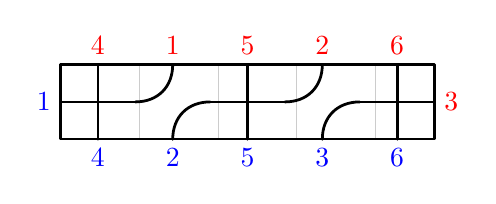
\begin{tikzpicture}[x=0.95cm,y=0.95cm,line cap=round,line join=round]
  % One-row grid paper
  \draw[gray!40, very thin] (0,0) grid (5,1);
  \draw[black, line width=0.8pt] (0,0) rectangle (5,1);

  % Cross tiles (plus shape, edge-center to edge-center)
  \foreach \c in {0,2,4}{
    \draw[line width=1.0pt] (\c,0.5) -- (\c+1,0.5);
    \draw[line width=1.0pt] (\c+0.5,0) -- (\c+0.5,1);
  }

  % Bump tiles (west->north and south->east)
  \foreach \c in {1,3}{
    \draw[line width=1.0pt] (\c+0.5,0) .. controls (\c+0.5,0.3) and (\c+0.7,0.5) .. (\c+1,0.5);
    \draw[line width=1.0pt] (\c,0.5) .. controls (\c+0.3,0.5) and (\c+0.5,0.7) .. (\c+0.5,1);
  }

  % Input labels (left and bottom)
  \node[left, text=blue] at (0,0.5) {$1$};
  \node[below, text=blue] at (0.5,0) {$4$};
  \node[below, text=blue] at (1.5,0) {$2$};
  \node[below, text=blue] at (2.5,0) {$5$};
  \node[below, text=blue] at (3.5,0) {$3$};
  \node[below, text=blue] at (4.5,0) {$6$};

  % Output labels after tracing strands (top, then right edge)
  \node[above, text=red] at (0.5,1) {$4$};
  \node[above, text=red] at (1.5,1) {$1$};
  \node[above, text=red] at (2.5,1) {$5$};
  \node[above, text=red] at (3.5,1) {$2$};
  \node[above, text=red] at (4.5,1) {$6$};
  \node[right, text=red] at (5,0.5) {$3$};
\end{tikzpicture}
\end{center}

Follow the strands through the row. The admissibility condition is that it cannot undo inversions, only create new ones.

\end{frame}

\begin{frame}{A nice combinatorial basis}
Let $\Xi_w^k$ be the basis indexed by permutations $w$ such that $w(p) < w(p+1)$ for all $p>k$ satisfying the following:
\begin{itemize}
\item $\Xi_{w}^1 = [w(1) - 1]$
\item For a nonnegative integer $[p]$, we have that
$$[p]\cdot\Xi_w^k = \sum_{w'}\Xi_{w'}^{k+1}$$
where $w'$ is obtained from $w$ through a valid crossing diagram with $p$ crosses after adding $1$ to each element of $w$ and adding a new first element $1$. 
\end{itemize}

I can provide an explicit (but mildly cancellative) formula for $\Xi_w^k$ in the word basis, as well as a positive formula for the product of $\Xi_u^p$ and $\Xi_v^q$ in terms of crossing diagrams. 

The coproduct structure constants are also nonnegative integers, but I do not have a positive combinatorial formula for them yet$\ldots$
\end{frame}

\begin{frame}{Taking off the mask: The dual Schubert basis}
The basis satisfies
$$\langle \mathfrak{S}_{u}(x_1,\ldots,x_n), \Xi_{v}^{n} \rangle = \delta_{u,v}$$
where $\mathfrak{S}_{u}(x_1,\ldots,x_n)$ is the Schubert polynomial corresponding to the permutation $u$.

The coefficients $c_{u,v}^{w}$ of the coproduct formula
\[
\Delta\,\Sch{w}^{n} = \sum_{u,v} c_{u,v}^{w}\,\Sch{u}^{n}\otimes \Sch{v}^{n}
\]

are the Littlewood-Richardson coefficients for Schubert polynomials!

\end{frame}

\begin{frame}{Solution of the classical LR problem}
  \begin{itemize}
  \item One solution of the classical LR problem (positive, combinatorial formula for multiplying Schur polynomials) is the associative algebra goverened by the Knuth relations on words of tableaux (Lascoux and Sch\"utzenberger, 1981 \cite{lascoux1981monoide}).
  \item This combinatorial construction creates an algebra with clearly nonnegative structure constants
  \item The subalgebra generated by sums of tableaux of a given shape behave precisely like the Schur polynomials, giving the solution

  \item I will do this here for dual Schubert polynomials!
  \end{itemize}
\end{frame}

% \begin{frame}{Coefficients of the dual Schubert basis}
%   For each $p$, define a relation on permutations
%   $$u\xrightarrow{p} v$$
%   If there is a $k+1$ cycle $c$ containing $p$ such that $v = uc$ and $\ell(v) = \ell(u) + k$. Define $\sigma_p(u,v)$ to be the number of elements of $c$ that are less than $p$.

% Then we have the following formula for the coefficients of $\Xi_w^k$ in the word basis:
% \begin{theorem}
% For each $w$, there is a permutation $\mu$ such that
% $$\Xi_w^k = \sum_{P=w^{-1}=w_0\xrightarrow{1} \cdots\xrightarrow{k}w_k=\mu} (-1)^{\sigma(P)}\wb{\mathrm{wt}(P)}$$
% where $\mathrm{wt}(P) = (\ell(1,u_1),\ldots,\ell(u_{k-1},u_k))$.
% \end{theorem}

% \end{frame}

% \begin{frame}{Theorem (placeholder): explicit LR rule in the dual Schubert basis}
% \textbf{Theorem.} \emph{(Placeholder for final statement.)}

% There is an explicit Littlewood--Richardson type rule for the concatenation product in the dual Schubert basis:
% \[
% \Sch{u}^{n_1}\cdot \Sch{v}^{n_2}
% =
% \sum_{w} c_{u,v}^{w}\,\Sch{w}^{n_1 + n_2},
% \]
% where $c_{u,v}^{w}$ are given by an explicit combinatorial counting rule.

% \vspace{0.5em}
% \textbf{To fill in during talk prep:}
% \begin{itemize}
%   \item precise combinatorial objects,
%   \item admissibility conditions,
%   \item exact indexing conventions.
% \end{itemize}
% \end{frame}

\begin{frame}{Bounded pipe dreams}
Pipe dreams are well-studied objects introduced in the $1990$s by Bergeron and Billey to give a nicer combinatorial formula for Schubert polynomials equivalent to an earlier one by Billey, Jockusch, and Stanley involving reduced words/compatible sequences.
\begin{center}
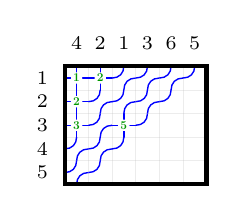
\begin{tikzpicture}[scale=0.3]
  \draw[lightgray, very thin, opacity=0.3] (0,1) -- (6,1);
  \draw[lightgray, very thin, opacity=0.3] (0,2) -- (6,2);
  \draw[lightgray, very thin, opacity=0.3] (0,3) -- (6,3);
  \draw[lightgray, very thin, opacity=0.3] (0,4) -- (6,4);
  \draw[lightgray, very thin, opacity=0.3] (0,5) -- (6,5);
  \draw[lightgray, very thin, opacity=0.3] (0,6) -- (6,6);
  \draw[lightgray, very thin, opacity=0.3] (0,1) -- (0,6);
  \draw[lightgray, very thin, opacity=0.3] (1,1) -- (1,6);
  \draw[lightgray, very thin, opacity=0.3] (2,1) -- (2,6);
  \draw[lightgray, very thin, opacity=0.3] (3,1) -- (3,6);
  \draw[lightgray, very thin, opacity=0.3] (4,1) -- (4,6);
  \draw[lightgray, very thin, opacity=0.3] (5,1) -- (5,6);
  \draw[lightgray, very thin, opacity=0.3] (6,1) -- (6,6);
  \draw[blue, line width=0.5pt, line cap=round] (0,5.5) -- (1,5.5);
  \draw[blue, line width=0.5pt, line cap=round] (0.5,5) -- (0.5,6);
  \draw[blue, line width=0.5pt, line cap=round] (1,5.5) -- (2,5.5);
  \draw[blue, line width=0.5pt, line cap=round] (1.5,5) -- (1.5,6);
  \draw[blue, line width=0.5pt] (2,5.5) .. controls (2.3,5.5) and (2.5,5.7) .. (2.5,6);
  \draw[blue, line width=0.5pt] (2.5,5) .. controls (2.5,5.3) and (2.7,5.5) .. (3,5.5);
  \draw[blue, line width=0.5pt] (3,5.5) .. controls (3.3,5.5) and (3.5,5.7) .. (3.5,6);
  \draw[blue, line width=0.5pt] (3.5,5) .. controls (3.5,5.3) and (3.7,5.5) .. (4,5.5);
  \draw[blue, line width=0.5pt] (4,5.5) .. controls (4.3,5.5) and (4.5,5.7) .. (4.5,6);
  \draw[blue, line width=0.5pt] (4.5,5) .. controls (4.5,5.3) and (4.7,5.5) .. (5,5.5);
  \draw[blue, line width=0.5pt] (5,5.5) .. controls (5.3,5.5) and (5.5,5.7) .. (5.5,6);
  \draw[blue, line width=0.5pt, line cap=round] (0,4.5) -- (1,4.5);
  \draw[blue, line width=0.5pt, line cap=round] (0.5,4) -- (0.5,5);
  \draw[blue, line width=0.5pt] (1,4.5) .. controls (1.3,4.5) and (1.5,4.7) .. (1.5,5);
  \draw[blue, line width=0.5pt] (1.5,4) .. controls (1.5,4.3) and (1.7,4.5) .. (2,4.5);
  \draw[blue, line width=0.5pt] (2,4.5) .. controls (2.3,4.5) and (2.5,4.7) .. (2.5,5);
  \draw[blue, line width=0.5pt] (2.5,4) .. controls (2.5,4.3) and (2.7,4.5) .. (3,4.5);
  \draw[blue, line width=0.5pt] (3,4.5) .. controls (3.3,4.5) and (3.5,4.7) .. (3.5,5);
  \draw[blue, line width=0.5pt] (3.5,4) .. controls (3.5,4.3) and (3.7,4.5) .. (4,4.5);
  \draw[blue, line width=0.5pt] (4,4.5) .. controls (4.3,4.5) and (4.5,4.7) .. (4.5,5);
  \draw[blue, line width=0.5pt, line cap=round] (0,3.5) -- (1,3.5);
  \draw[blue, line width=0.5pt, line cap=round] (0.5,3) -- (0.5,4);
  \draw[blue, line width=0.5pt] (1,3.5) .. controls (1.3,3.5) and (1.5,3.7) .. (1.5,4);
  \draw[blue, line width=0.5pt] (1.5,3) .. controls (1.5,3.3) and (1.7,3.5) .. (2,3.5);
  \draw[blue, line width=0.5pt, line cap=round] (2,3.5) -- (3,3.5);
  \draw[blue, line width=0.5pt, line cap=round] (2.5,3) -- (2.5,4);
  \draw[blue, line width=0.5pt] (3,3.5) .. controls (3.3,3.5) and (3.5,3.7) .. (3.5,4);
  \draw[blue, line width=0.5pt] (0,2.5) .. controls (0.3,2.5) and (0.5,2.7) .. (0.5,3);
  \draw[blue, line width=0.5pt] (0.5,2) .. controls (0.5,2.3) and (0.7,2.5) .. (1,2.5);
  \draw[blue, line width=0.5pt] (1,2.5) .. controls (1.3,2.5) and (1.5,2.7) .. (1.5,3);
  \draw[blue, line width=0.5pt] (1.5,2) .. controls (1.5,2.3) and (1.7,2.5) .. (2,2.5);
  \draw[blue, line width=0.5pt] (2,2.5) .. controls (2.3,2.5) and (2.5,2.7) .. (2.5,3);
  \draw[blue, line width=0.5pt] (0,1.5) .. controls (0.3,1.5) and (0.5,1.7) .. (0.5,2);
  \draw[blue, line width=0.5pt] (0.5,1) .. controls (0.5,1.3) and (0.7,1.5) .. (1,1.5);
  \draw[blue, line width=0.5pt] (1,1.5) .. controls (1.3,1.5) and (1.5,1.7) .. (1.5,2);
  \node[font=\Large\bfseries, text=green!60!black, fill=white, inner sep=0.5pt, circle, transform shape] at (1.5,5.5) {2};
  \node[font=\Large\bfseries, text=green!60!black, fill=white, inner sep=0.5pt, circle, transform shape] at (0.5,4.5) {2};
  \node[font=\Large\bfseries, text=green!60!black, fill=white, inner sep=0.5pt, circle, transform shape] at (0.5,3.5) {3};
  \node[font=\Large\bfseries, text=green!60!black, fill=white, inner sep=0.5pt, circle, transform shape] at (0.5,5.5) {1};
  \node[font=\Large\bfseries, text=green!60!black, fill=white, inner sep=0.5pt, circle, transform shape] at (2.5,3.5) {5};
  \node[font=\scriptsize, text=black, anchor=south] at (0.5,6.3) {4};
  \node[font=\scriptsize, text=black, anchor=south] at (1.5,6.3) {2};
  \node[font=\scriptsize, text=black, anchor=south] at (2.5,6.3) {1};
  \node[font=\scriptsize, text=black, anchor=south] at (3.5,6.3) {3};
  \node[font=\scriptsize, text=black, anchor=south] at (4.5,6.3) {6};
  \node[font=\scriptsize, text=black, anchor=south] at (5.5,6.3) {5};
  \node[font=\scriptsize, text=black, anchor=east] at (-0.3,5.5) {1};
  \node[font=\scriptsize, text=black, anchor=east] at (-0.3,4.5) {2};
  \node[font=\scriptsize, text=black, anchor=east] at (-0.3,3.5) {3};
  \node[font=\scriptsize, text=black, anchor=east] at (-0.3,2.5) {4};
  \node[font=\scriptsize, text=black, anchor=east] at (-0.3,1.5) {5};
  \draw[black, line width=1.5pt] (0,1) rectangle (6,6);
\end{tikzpicture}
\end{center}

\begin{theorem}[Bergeron, Billey, 1993 \cite{bbrc}]
The Schubert polynomial $\mathfrak{S}_w$ is equal to
$$\sum_{R\in\RC(w)}x_{\mathrm{wt}(R)}$$
where $\RC(w)$ is the set of pipe dreams with permutation $w$ and $\mathrm{wt}(R)$ is the weak composition whose $i$-th part is the number of crosses in row $i$ of $R$.
\end{theorem}


\end{frame}

\begin{frame}{Transition algorithm on bounded pipe dreams}
  There is an algorithm that takes a bounded pipe dream of length $n$ with row $n$ empty to a unique pipe dream of length $n-1$
in a way that matches the Schubert transition formula in a strong, weight-preserving, structure-preserving form.
\begin{center}
  {\scriptsize
  \begin{algorithmic}
		\State \textbf{Input:} A bounded pipe dream $R$ with $\hr(R)=n$ and row $n$ empty.
		\State \textbf{Output:} A bounded  pipe dream $R'$ with $\hr(R')=n-1$, $|R'|=|R|$ (same number of crossing in each row), and $\wof{R}\downvar{n} \wof{R'}$.
		
		\If{$R$ with last row removed is a valid bounded pipe dream}
		\State \Return $R$ with last row removed
		\Else
		\State Locate crossings corresponding to maximal right descents of $w(R)$ until the maximal right descent is $n-1$, say at rows $i_1 < i_2 < \cdots < i_p$ with corresponding columns $j_1, j_2, \ldots, j_p$.
		\State $R^- \gets R \setminus \{(i_1, j_1), \ldots, (i_p, j_p)\}$.
		\State Let $I \gets (i_1, i_2, \ldots, i_p)$.
		\State $D \gets R^- \cup \{(n, 1), (n, 2), \ldots, (n, p)\}$.
		\State $D' \gets \ins{n-1}{I} D$ (an insertion algorithm similar to existing ones for pipe dreams)
		\State $R' \gets \{(i, j) \in D' \mid i < n\}$ as a bounded pipe dream with $n-1$ rows.
		\State \Return $R'$.
		\EndIf
	\end{algorithmic}
  }
\end{center}
\end{frame}

\begin{frame}{Bounded pipe dream ring product}
Given bounded pipe dreams $R_1,R_2$, define $R_1\star R_2$ by taking the sum of all $R$ obtained by
\begin{itemize}
  \item \emph{untransitioning} $R_1$ in all possible valid ways to create space while remaining a pipe dream,
  \item shifting $R_2$ downward,
  \item placing the shifted $R_2$ into the new empty region, unchanged, if doing so yields a valid pipe dream.
\end{itemize}
This allows us to lift the product of the dual algebra $\dcoma$ to a product on formal linear combinations of bounded pipe dreams.
\begin{theorem}[S, 2026+]
The product $\star$ is associative and gives a well-defined ring structure on the vector space $\RC$ spanned by bounded pipe dreams.
\end{theorem}
\end{frame}

\begin{frame}{Product example}
  \centering
  \begin{minipage}{0.45\textwidth}\centering
  $rc$\\[0.3em]
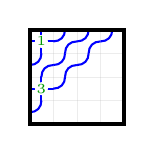
\begin{tikzpicture}[scale=0.3]
  \draw[lightgray, very thin, opacity=0.3] (0,0) -- (4,0);
  \draw[lightgray, very thin, opacity=0.3] (0,0) -- (0,4);
  \draw[lightgray, very thin, opacity=0.3] (0,1) -- (4,1);
  \draw[lightgray, very thin, opacity=0.3] (1,0) -- (1,4);
  \draw[lightgray, very thin, opacity=0.3] (0,2) -- (4,2);
  \draw[lightgray, very thin, opacity=0.3] (2,0) -- (2,4);
  \draw[lightgray, very thin, opacity=0.3] (0,3) -- (4,3);
  \draw[lightgray, very thin, opacity=0.3] (3,0) -- (3,4);
  \draw[lightgray, very thin, opacity=0.3] (0,4) -- (4,4);
  \draw[lightgray, very thin, opacity=0.3] (4,0) -- (4,4);
  \draw[blue, line width=0.75pt, line cap=round] (0,3.5) -- (1,3.5);
  \draw[blue, line width=0.75pt, line cap=round] (0.5,3) -- (0.5,4);
  \draw[blue, line width=0.75pt] (1,3.5) .. controls (1.3,3.5) and (1.5,3.7) .. (1.5,4);
  \draw[blue, line width=0.75pt] (1.5,3) .. controls (1.5,3.3) and (1.7,3.5) .. (2,3.5);
  \draw[blue, line width=0.75pt] (2,3.5) .. controls (2.3,3.5) and (2.5,3.7) .. (2.5,4);
  \draw[blue, line width=0.75pt] (2.5,3) .. controls (2.5,3.3) and (2.7,3.5) .. (3,3.5);
  \draw[blue, line width=0.75pt] (3,3.5) .. controls (3.3,3.5) and (3.5,3.7) .. (3.5,4);
  \draw[blue, line width=0.75pt] (0,2.5) .. controls (0.3,2.5) and (0.5,2.7) .. (0.5,3);
  \draw[blue, line width=0.75pt] (0.5,2) .. controls (0.5,2.3) and (0.7,2.5) .. (1,2.5);
  \draw[blue, line width=0.75pt] (1,2.5) .. controls (1.3,2.5) and (1.5,2.7) .. (1.5,3);
  \draw[blue, line width=0.75pt] (1.5,2) .. controls (1.5,2.3) and (1.7,2.5) .. (2,2.5);
  \draw[blue, line width=0.75pt] (2,2.5) .. controls (2.3,2.5) and (2.5,2.7) .. (2.5,3);
  \draw[blue, line width=0.75pt, line cap=round] (0,1.5) -- (1,1.5);
  \draw[blue, line width=0.75pt, line cap=round] (0.5,1) -- (0.5,2);
  \draw[blue, line width=0.75pt] (1,1.5) .. controls (1.3,1.5) and (1.5,1.7) .. (1.5,2);
  \draw[blue, line width=0.75pt] (0,0.5) .. controls (0.3,0.5) and (0.5,0.7) .. (0.5,1);
  \node[font=\fontsize{3}{3}\selectfont, text=green!60!black, fill=white, inner sep=0pt, circle] at (0.5,1.5) {3};
  \node[font=\fontsize{3}{3}\selectfont, text=green!60!black, fill=white, inner sep=0pt, circle] at (0.5,3.5) {1};
  \draw[black, line width=1.4pt] (0,0) rectangle (4,4);
\end{tikzpicture}
  \end{minipage}
  $\star$
  \begin{minipage}{0.45\textwidth}\centering
  $rc_2$\\[0.3em]
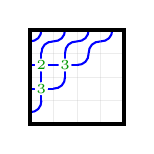
\begin{tikzpicture}[scale=0.3]
  \draw[lightgray, very thin, opacity=0.3] (0,0) -- (4,0);
  \draw[lightgray, very thin, opacity=0.3] (0,0) -- (0,4);
  \draw[lightgray, very thin, opacity=0.3] (0,1) -- (4,1);
  \draw[lightgray, very thin, opacity=0.3] (1,0) -- (1,4);
  \draw[lightgray, very thin, opacity=0.3] (0,2) -- (4,2);
  \draw[lightgray, very thin, opacity=0.3] (2,0) -- (2,4);
  \draw[lightgray, very thin, opacity=0.3] (0,3) -- (4,3);
  \draw[lightgray, very thin, opacity=0.3] (3,0) -- (3,4);
  \draw[lightgray, very thin, opacity=0.3] (0,4) -- (4,4);
  \draw[lightgray, very thin, opacity=0.3] (4,0) -- (4,4);
  \draw[blue, line width=0.75pt] (0,3.5) .. controls (0.3,3.5) and (0.5,3.7) .. (0.5,4);
  \draw[blue, line width=0.75pt] (0.5,3) .. controls (0.5,3.3) and (0.7,3.5) .. (1,3.5);
  \draw[blue, line width=0.75pt] (1,3.5) .. controls (1.3,3.5) and (1.5,3.7) .. (1.5,4);
  \draw[blue, line width=0.75pt] (1.5,3) .. controls (1.5,3.3) and (1.7,3.5) .. (2,3.5);
  \draw[blue, line width=0.75pt] (2,3.5) .. controls (2.3,3.5) and (2.5,3.7) .. (2.5,4);
  \draw[blue, line width=0.75pt] (2.5,3) .. controls (2.5,3.3) and (2.7,3.5) .. (3,3.5);
  \draw[blue, line width=0.75pt] (3,3.5) .. controls (3.3,3.5) and (3.5,3.7) .. (3.5,4);
  \draw[blue, line width=0.75pt, line cap=round] (0,2.5) -- (1,2.5);
  \draw[blue, line width=0.75pt, line cap=round] (0.5,2) -- (0.5,3);
  \draw[blue, line width=0.75pt, line cap=round] (1,2.5) -- (2,2.5);
  \draw[blue, line width=0.75pt, line cap=round] (1.5,2) -- (1.5,3);
  \draw[blue, line width=0.75pt] (2,2.5) .. controls (2.3,2.5) and (2.5,2.7) .. (2.5,3);
  \draw[blue, line width=0.75pt, line cap=round] (0,1.5) -- (1,1.5);
  \draw[blue, line width=0.75pt, line cap=round] (0.5,1) -- (0.5,2);
  \draw[blue, line width=0.75pt] (1,1.5) .. controls (1.3,1.5) and (1.5,1.7) .. (1.5,2);
  \draw[blue, line width=0.75pt] (0,0.5) .. controls (0.3,0.5) and (0.5,0.7) .. (0.5,1);
  \node[font=\fontsize{3}{3}\selectfont, text=green!60!black, fill=white, inner sep=0pt, circle] at (0.5,1.5) {3};
  \node[font=\fontsize{3}{3}\selectfont, text=green!60!black, fill=white, inner sep=0pt, circle] at (0.5,2.5) {2};
  \node[font=\fontsize{3}{3}\selectfont, text=green!60!black, fill=white, inner sep=0pt, circle] at (1.5,2.5) {3};
  \draw[black, line width=1.4pt] (0,0) rectangle (4,4);
\end{tikzpicture}
  \end{minipage}

  \vspace{0.5em}
  \textit{Untransitioning of $rc$}

  \vspace{0.3em}
  \begin{minipage}{0.18\textwidth}\centering\scriptsize A\\[0.2em]
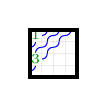
\begin{tikzpicture}[scale=0.15]
  \draw[lightgray, very thin, opacity=0.3] (0,0) -- (4,0);
  \draw[lightgray, very thin, opacity=0.3] (0,0) -- (0,4);
  \draw[lightgray, very thin, opacity=0.3] (0,1) -- (4,1);
  \draw[lightgray, very thin, opacity=0.3] (1,0) -- (1,4);
  \draw[lightgray, very thin, opacity=0.3] (0,2) -- (4,2);
  \draw[lightgray, very thin, opacity=0.3] (2,0) -- (2,4);
  \draw[lightgray, very thin, opacity=0.3] (0,3) -- (4,3);
  \draw[lightgray, very thin, opacity=0.3] (3,0) -- (3,4);
  \draw[lightgray, very thin, opacity=0.3] (0,4) -- (4,4);
  \draw[lightgray, very thin, opacity=0.3] (4,0) -- (4,4);
  \draw[blue, line width=0.375pt, line cap=round] (0,3.5) -- (1,3.5);
  \draw[blue, line width=0.375pt, line cap=round] (0.5,3) -- (0.5,4);
  \draw[blue, line width=0.375pt] (1,3.5) .. controls (1.3,3.5) and (1.5,3.7) .. (1.5,4);
  \draw[blue, line width=0.375pt] (1.5,3) .. controls (1.5,3.3) and (1.7,3.5) .. (2,3.5);
  \draw[blue, line width=0.375pt] (2,3.5) .. controls (2.3,3.5) and (2.5,3.7) .. (2.5,4);
  \draw[blue, line width=0.375pt] (2.5,3) .. controls (2.5,3.3) and (2.7,3.5) .. (3,3.5);
  \draw[blue, line width=0.375pt] (3,3.5) .. controls (3.3,3.5) and (3.5,3.7) .. (3.5,4);
  \draw[blue, line width=0.375pt] (0,2.5) .. controls (0.3,2.5) and (0.5,2.7) .. (0.5,3);
  \draw[blue, line width=0.375pt] (0.5,2) .. controls (0.5,2.3) and (0.7,2.5) .. (1,2.5);
  \draw[blue, line width=0.375pt] (1,2.5) .. controls (1.3,2.5) and (1.5,2.7) .. (1.5,3);
  \draw[blue, line width=0.375pt] (1.5,2) .. controls (1.5,2.3) and (1.7,2.5) .. (2,2.5);
  \draw[blue, line width=0.375pt] (2,2.5) .. controls (2.3,2.5) and (2.5,2.7) .. (2.5,3);
  \draw[blue, line width=0.375pt, line cap=round] (0,1.5) -- (1,1.5);
  \draw[blue, line width=0.375pt, line cap=round] (0.5,1) -- (0.5,2);
  \draw[blue, line width=0.375pt] (1,1.5) .. controls (1.3,1.5) and (1.5,1.7) .. (1.5,2);
  \draw[blue, line width=0.375pt] (0,0.5) .. controls (0.3,0.5) and (0.5,0.7) .. (0.5,1);
  \node[font=\fontsize{3}{3}\selectfont, text=green!60!black, fill=white, inner sep=0pt, circle] at (0.5,1.5) {3};
  \node[font=\fontsize{3}{3}\selectfont, text=green!60!black, fill=white, inner sep=0pt, circle] at (0.5,3.5) {1};
  \draw[black, line width=1.4pt] (0,0) rectangle (4,4);
\end{tikzpicture}
  \end{minipage}
  \begin{minipage}{0.18\textwidth}\centering\scriptsize B\\[0.2em]
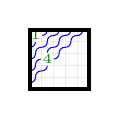
\begin{tikzpicture}[scale=0.15]
  \draw[lightgray, very thin, opacity=0.3] (0,0) -- (5,0);
  \draw[lightgray, very thin, opacity=0.3] (0,0) -- (0,5);
  \draw[lightgray, very thin, opacity=0.3] (0,1) -- (5,1);
  \draw[lightgray, very thin, opacity=0.3] (1,0) -- (1,5);
  \draw[lightgray, very thin, opacity=0.3] (0,2) -- (5,2);
  \draw[lightgray, very thin, opacity=0.3] (2,0) -- (2,5);
  \draw[lightgray, very thin, opacity=0.3] (0,3) -- (5,3);
  \draw[lightgray, very thin, opacity=0.3] (3,0) -- (3,5);
  \draw[lightgray, very thin, opacity=0.3] (0,4) -- (5,4);
  \draw[lightgray, very thin, opacity=0.3] (4,0) -- (4,5);
  \draw[lightgray, very thin, opacity=0.3] (0,5) -- (5,5);
  \draw[lightgray, very thin, opacity=0.3] (5,0) -- (5,5);
  \draw[blue, line width=0.375pt, line cap=round] (0,4.5) -- (1,4.5);
  \draw[blue, line width=0.375pt, line cap=round] (0.5,4) -- (0.5,5);
  \draw[blue, line width=0.375pt] (1,4.5) .. controls (1.3,4.5) and (1.5,4.7) .. (1.5,5);
  \draw[blue, line width=0.375pt] (1.5,4) .. controls (1.5,4.3) and (1.7,4.5) .. (2,4.5);
  \draw[blue, line width=0.375pt] (2,4.5) .. controls (2.3,4.5) and (2.5,4.7) .. (2.5,5);
  \draw[blue, line width=0.375pt] (2.5,4) .. controls (2.5,4.3) and (2.7,4.5) .. (3,4.5);
  \draw[blue, line width=0.375pt] (3,4.5) .. controls (3.3,4.5) and (3.5,4.7) .. (3.5,5);
  \draw[blue, line width=0.375pt] (3.5,4) .. controls (3.5,4.3) and (3.7,4.5) .. (4,4.5);
  \draw[blue, line width=0.375pt] (4,4.5) .. controls (4.3,4.5) and (4.5,4.7) .. (4.5,5);
  \draw[blue, line width=0.375pt] (0,3.5) .. controls (0.3,3.5) and (0.5,3.7) .. (0.5,4);
  \draw[blue, line width=0.375pt] (0.5,3) .. controls (0.5,3.3) and (0.7,3.5) .. (1,3.5);
  \draw[blue, line width=0.375pt] (1,3.5) .. controls (1.3,3.5) and (1.5,3.7) .. (1.5,4);
  \draw[blue, line width=0.375pt] (1.5,3) .. controls (1.5,3.3) and (1.7,3.5) .. (2,3.5);
  \draw[blue, line width=0.375pt] (2,3.5) .. controls (2.3,3.5) and (2.5,3.7) .. (2.5,4);
  \draw[blue, line width=0.375pt] (2.5,3) .. controls (2.5,3.3) and (2.7,3.5) .. (3,3.5);
  \draw[blue, line width=0.375pt] (3,3.5) .. controls (3.3,3.5) and (3.5,3.7) .. (3.5,4);
  \draw[blue, line width=0.375pt] (0,2.5) .. controls (0.3,2.5) and (0.5,2.7) .. (0.5,3);
  \draw[blue, line width=0.375pt] (0.5,2) .. controls (0.5,2.3) and (0.7,2.5) .. (1,2.5);
  \draw[blue, line width=0.375pt, line cap=round] (1,2.5) -- (2,2.5);
  \draw[blue, line width=0.375pt, line cap=round] (1.5,2) -- (1.5,3);
  \draw[blue, line width=0.375pt] (2,2.5) .. controls (2.3,2.5) and (2.5,2.7) .. (2.5,3);
  \draw[blue, line width=0.375pt] (0,1.5) .. controls (0.3,1.5) and (0.5,1.7) .. (0.5,2);
  \draw[blue, line width=0.375pt] (0.5,1) .. controls (0.5,1.3) and (0.7,1.5) .. (1,1.5);
  \draw[blue, line width=0.375pt] (1,1.5) .. controls (1.3,1.5) and (1.5,1.7) .. (1.5,2);
  \draw[blue, line width=0.375pt] (0,0.5) .. controls (0.3,0.5) and (0.5,0.7) .. (0.5,1);
  \node[font=\fontsize{3}{3}\selectfont, text=green!60!black, fill=white, inner sep=0pt, circle] at (0.5,4.5) {1};
  \node[font=\fontsize{3}{3}\selectfont, text=green!60!black, fill=white, inner sep=0pt, circle] at (1.5,2.5) {4};
  \draw[black, line width=1.4pt] (0,0) rectangle (5,5);
\end{tikzpicture}
  \end{minipage}
  \begin{minipage}{0.18\textwidth}\centering\scriptsize C\\[0.2em]
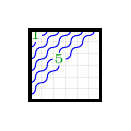
\begin{tikzpicture}[scale=0.15]
  \draw[lightgray, very thin, opacity=0.3] (0,0) -- (6,0);
  \draw[lightgray, very thin, opacity=0.3] (0,0) -- (0,6);
  \draw[lightgray, very thin, opacity=0.3] (0,1) -- (6,1);
  \draw[lightgray, very thin, opacity=0.3] (1,0) -- (1,6);
  \draw[lightgray, very thin, opacity=0.3] (0,2) -- (6,2);
  \draw[lightgray, very thin, opacity=0.3] (2,0) -- (2,6);
  \draw[lightgray, very thin, opacity=0.3] (0,3) -- (6,3);
  \draw[lightgray, very thin, opacity=0.3] (3,0) -- (3,6);
  \draw[lightgray, very thin, opacity=0.3] (0,4) -- (6,4);
  \draw[lightgray, very thin, opacity=0.3] (4,0) -- (4,6);
  \draw[lightgray, very thin, opacity=0.3] (0,5) -- (6,5);
  \draw[lightgray, very thin, opacity=0.3] (5,0) -- (5,6);
  \draw[lightgray, very thin, opacity=0.3] (0,6) -- (6,6);
  \draw[lightgray, very thin, opacity=0.3] (6,0) -- (6,6);
  \draw[blue, line width=0.375pt, line cap=round] (0,5.5) -- (1,5.5);
  \draw[blue, line width=0.375pt, line cap=round] (0.5,5) -- (0.5,6);
  \draw[blue, line width=0.375pt] (1,5.5) .. controls (1.3,5.5) and (1.5,5.7) .. (1.5,6);
  \draw[blue, line width=0.375pt] (1.5,5) .. controls (1.5,5.3) and (1.7,5.5) .. (2,5.5);
  \draw[blue, line width=0.375pt] (2,5.5) .. controls (2.3,5.5) and (2.5,5.7) .. (2.5,6);
  \draw[blue, line width=0.375pt] (2.5,5) .. controls (2.5,5.3) and (2.7,5.5) .. (3,5.5);
  \draw[blue, line width=0.375pt] (3,5.5) .. controls (3.3,5.5) and (3.5,5.7) .. (3.5,6);
  \draw[blue, line width=0.375pt] (3.5,5) .. controls (3.5,5.3) and (3.7,5.5) .. (4,5.5);
  \draw[blue, line width=0.375pt] (4,5.5) .. controls (4.3,5.5) and (4.5,5.7) .. (4.5,6);
  \draw[blue, line width=0.375pt] (4.5,5) .. controls (4.5,5.3) and (4.7,5.5) .. (5,5.5);
  \draw[blue, line width=0.375pt] (5,5.5) .. controls (5.3,5.5) and (5.5,5.7) .. (5.5,6);
  \draw[blue, line width=0.375pt] (0,4.5) .. controls (0.3,4.5) and (0.5,4.7) .. (0.5,5);
  \draw[blue, line width=0.375pt] (0.5,4) .. controls (0.5,4.3) and (0.7,4.5) .. (1,4.5);
  \draw[blue, line width=0.375pt] (1,4.5) .. controls (1.3,4.5) and (1.5,4.7) .. (1.5,5);
  \draw[blue, line width=0.375pt] (1.5,4) .. controls (1.5,4.3) and (1.7,4.5) .. (2,4.5);
  \draw[blue, line width=0.375pt] (2,4.5) .. controls (2.3,4.5) and (2.5,4.7) .. (2.5,5);
  \draw[blue, line width=0.375pt] (2.5,4) .. controls (2.5,4.3) and (2.7,4.5) .. (3,4.5);
  \draw[blue, line width=0.375pt] (3,4.5) .. controls (3.3,4.5) and (3.5,4.7) .. (3.5,5);
  \draw[blue, line width=0.375pt] (3.5,4) .. controls (3.5,4.3) and (3.7,4.5) .. (4,4.5);
  \draw[blue, line width=0.375pt] (4,4.5) .. controls (4.3,4.5) and (4.5,4.7) .. (4.5,5);
  \draw[blue, line width=0.375pt] (0,3.5) .. controls (0.3,3.5) and (0.5,3.7) .. (0.5,4);
  \draw[blue, line width=0.375pt] (0.5,3) .. controls (0.5,3.3) and (0.7,3.5) .. (1,3.5);
  \draw[blue, line width=0.375pt] (1,3.5) .. controls (1.3,3.5) and (1.5,3.7) .. (1.5,4);
  \draw[blue, line width=0.375pt] (1.5,3) .. controls (1.5,3.3) and (1.7,3.5) .. (2,3.5);
  \draw[blue, line width=0.375pt, line cap=round] (2,3.5) -- (3,3.5);
  \draw[blue, line width=0.375pt, line cap=round] (2.5,3) -- (2.5,4);
  \draw[blue, line width=0.375pt] (3,3.5) .. controls (3.3,3.5) and (3.5,3.7) .. (3.5,4);
  \draw[blue, line width=0.375pt] (0,2.5) .. controls (0.3,2.5) and (0.5,2.7) .. (0.5,3);
  \draw[blue, line width=0.375pt] (0.5,2) .. controls (0.5,2.3) and (0.7,2.5) .. (1,2.5);
  \draw[blue, line width=0.375pt] (1,2.5) .. controls (1.3,2.5) and (1.5,2.7) .. (1.5,3);
  \draw[blue, line width=0.375pt] (1.5,2) .. controls (1.5,2.3) and (1.7,2.5) .. (2,2.5);
  \draw[blue, line width=0.375pt] (2,2.5) .. controls (2.3,2.5) and (2.5,2.7) .. (2.5,3);
  \draw[blue, line width=0.375pt] (0,1.5) .. controls (0.3,1.5) and (0.5,1.7) .. (0.5,2);
  \draw[blue, line width=0.375pt] (0.5,1) .. controls (0.5,1.3) and (0.7,1.5) .. (1,1.5);
  \draw[blue, line width=0.375pt] (1,1.5) .. controls (1.3,1.5) and (1.5,1.7) .. (1.5,2);
  \draw[blue, line width=0.375pt] (0,0.5) .. controls (0.3,0.5) and (0.5,0.7) .. (0.5,1);
  \node[font=\fontsize{3}{3}\selectfont, text=green!60!black, fill=white, inner sep=0pt, circle] at (0.5,5.5) {1};
  \node[font=\fontsize{3}{3}\selectfont, text=green!60!black, fill=white, inner sep=0pt, circle] at (2.5,3.5) {5};
  \draw[black, line width=1.4pt] (0,0) rectangle (6,6);
\end{tikzpicture}
  \end{minipage}
  \begin{minipage}{0.18\textwidth}\centering\scriptsize D\\[0.2em]
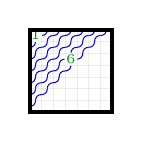
\begin{tikzpicture}[scale=0.15]
  \draw[lightgray, very thin, opacity=0.3] (0,0) -- (7,0);
  \draw[lightgray, very thin, opacity=0.3] (0,0) -- (0,7);
  \draw[lightgray, very thin, opacity=0.3] (0,1) -- (7,1);
  \draw[lightgray, very thin, opacity=0.3] (1,0) -- (1,7);
  \draw[lightgray, very thin, opacity=0.3] (0,2) -- (7,2);
  \draw[lightgray, very thin, opacity=0.3] (2,0) -- (2,7);
  \draw[lightgray, very thin, opacity=0.3] (0,3) -- (7,3);
  \draw[lightgray, very thin, opacity=0.3] (3,0) -- (3,7);
  \draw[lightgray, very thin, opacity=0.3] (0,4) -- (7,4);
  \draw[lightgray, very thin, opacity=0.3] (4,0) -- (4,7);
  \draw[lightgray, very thin, opacity=0.3] (0,5) -- (7,5);
  \draw[lightgray, very thin, opacity=0.3] (5,0) -- (5,7);
  \draw[lightgray, very thin, opacity=0.3] (0,6) -- (7,6);
  \draw[lightgray, very thin, opacity=0.3] (6,0) -- (6,7);
  \draw[lightgray, very thin, opacity=0.3] (0,7) -- (7,7);
  \draw[lightgray, very thin, opacity=0.3] (7,0) -- (7,7);
  \draw[blue, line width=0.375pt, line cap=round] (0,6.5) -- (1,6.5);
  \draw[blue, line width=0.375pt, line cap=round] (0.5,6) -- (0.5,7);
  \draw[blue, line width=0.375pt] (1,6.5) .. controls (1.3,6.5) and (1.5,6.7) .. (1.5,7);
  \draw[blue, line width=0.375pt] (1.5,6) .. controls (1.5,6.3) and (1.7,6.5) .. (2,6.5);
  \draw[blue, line width=0.375pt] (2,6.5) .. controls (2.3,6.5) and (2.5,6.7) .. (2.5,7);
  \draw[blue, line width=0.375pt] (2.5,6) .. controls (2.5,6.3) and (2.7,6.5) .. (3,6.5);
  \draw[blue, line width=0.375pt] (3,6.5) .. controls (3.3,6.5) and (3.5,6.7) .. (3.5,7);
  \draw[blue, line width=0.375pt] (3.5,6) .. controls (3.5,6.3) and (3.7,6.5) .. (4,6.5);
  \draw[blue, line width=0.375pt] (4,6.5) .. controls (4.3,6.5) and (4.5,6.7) .. (4.5,7);
  \draw[blue, line width=0.375pt] (4.5,6) .. controls (4.5,6.3) and (4.7,6.5) .. (5,6.5);
  \draw[blue, line width=0.375pt] (5,6.5) .. controls (5.3,6.5) and (5.5,6.7) .. (5.5,7);
  \draw[blue, line width=0.375pt] (5.5,6) .. controls (5.5,6.3) and (5.7,6.5) .. (6,6.5);
  \draw[blue, line width=0.375pt] (6,6.5) .. controls (6.3,6.5) and (6.5,6.7) .. (6.5,7);
  \draw[blue, line width=0.375pt] (0,5.5) .. controls (0.3,5.5) and (0.5,5.7) .. (0.5,6);
  \draw[blue, line width=0.375pt] (0.5,5) .. controls (0.5,5.3) and (0.7,5.5) .. (1,5.5);
  \draw[blue, line width=0.375pt] (1,5.5) .. controls (1.3,5.5) and (1.5,5.7) .. (1.5,6);
  \draw[blue, line width=0.375pt] (1.5,5) .. controls (1.5,5.3) and (1.7,5.5) .. (2,5.5);
  \draw[blue, line width=0.375pt] (2,5.5) .. controls (2.3,5.5) and (2.5,5.7) .. (2.5,6);
  \draw[blue, line width=0.375pt] (2.5,5) .. controls (2.5,5.3) and (2.7,5.5) .. (3,5.5);
  \draw[blue, line width=0.375pt] (3,5.5) .. controls (3.3,5.5) and (3.5,5.7) .. (3.5,6);
  \draw[blue, line width=0.375pt] (3.5,5) .. controls (3.5,5.3) and (3.7,5.5) .. (4,5.5);
  \draw[blue, line width=0.375pt] (4,5.5) .. controls (4.3,5.5) and (4.5,5.7) .. (4.5,6);
  \draw[blue, line width=0.375pt] (4.5,5) .. controls (4.5,5.3) and (4.7,5.5) .. (5,5.5);
  \draw[blue, line width=0.375pt] (5,5.5) .. controls (5.3,5.5) and (5.5,5.7) .. (5.5,6);
  \draw[blue, line width=0.375pt] (0,4.5) .. controls (0.3,4.5) and (0.5,4.7) .. (0.5,5);
  \draw[blue, line width=0.375pt] (0.5,4) .. controls (0.5,4.3) and (0.7,4.5) .. (1,4.5);
  \draw[blue, line width=0.375pt] (1,4.5) .. controls (1.3,4.5) and (1.5,4.7) .. (1.5,5);
  \draw[blue, line width=0.375pt] (1.5,4) .. controls (1.5,4.3) and (1.7,4.5) .. (2,4.5);
  \draw[blue, line width=0.375pt] (2,4.5) .. controls (2.3,4.5) and (2.5,4.7) .. (2.5,5);
  \draw[blue, line width=0.375pt] (2.5,4) .. controls (2.5,4.3) and (2.7,4.5) .. (3,4.5);
  \draw[blue, line width=0.375pt, line cap=round] (3,4.5) -- (4,4.5);
  \draw[blue, line width=0.375pt, line cap=round] (3.5,4) -- (3.5,5);
  \draw[blue, line width=0.375pt] (4,4.5) .. controls (4.3,4.5) and (4.5,4.7) .. (4.5,5);
  \draw[blue, line width=0.375pt] (0,3.5) .. controls (0.3,3.5) and (0.5,3.7) .. (0.5,4);
  \draw[blue, line width=0.375pt] (0.5,3) .. controls (0.5,3.3) and (0.7,3.5) .. (1,3.5);
  \draw[blue, line width=0.375pt] (1,3.5) .. controls (1.3,3.5) and (1.5,3.7) .. (1.5,4);
  \draw[blue, line width=0.375pt] (1.5,3) .. controls (1.5,3.3) and (1.7,3.5) .. (2,3.5);
  \draw[blue, line width=0.375pt] (2,3.5) .. controls (2.3,3.5) and (2.5,3.7) .. (2.5,4);
  \draw[blue, line width=0.375pt] (2.5,3) .. controls (2.5,3.3) and (2.7,3.5) .. (3,3.5);
  \draw[blue, line width=0.375pt] (3,3.5) .. controls (3.3,3.5) and (3.5,3.7) .. (3.5,4);
  \draw[blue, line width=0.375pt] (0,2.5) .. controls (0.3,2.5) and (0.5,2.7) .. (0.5,3);
  \draw[blue, line width=0.375pt] (0.5,2) .. controls (0.5,2.3) and (0.7,2.5) .. (1,2.5);
  \draw[blue, line width=0.375pt] (1,2.5) .. controls (1.3,2.5) and (1.5,2.7) .. (1.5,3);
  \draw[blue, line width=0.375pt] (1.5,2) .. controls (1.5,2.3) and (1.7,2.5) .. (2,2.5);
  \draw[blue, line width=0.375pt] (2,2.5) .. controls (2.3,2.5) and (2.5,2.7) .. (2.5,3);
  \draw[blue, line width=0.375pt] (0,1.5) .. controls (0.3,1.5) and (0.5,1.7) .. (0.5,2);
  \draw[blue, line width=0.375pt] (0.5,1) .. controls (0.5,1.3) and (0.7,1.5) .. (1,1.5);
  \draw[blue, line width=0.375pt] (1,1.5) .. controls (1.3,1.5) and (1.5,1.7) .. (1.5,2);
  \draw[blue, line width=0.375pt] (0,0.5) .. controls (0.3,0.5) and (0.5,0.7) .. (0.5,1);
  \node[font=\fontsize{3}{3}\selectfont, text=green!60!black, fill=white, inner sep=0pt, circle] at (0.5,6.5) {1};
  \node[font=\fontsize{3}{3}\selectfont, text=green!60!black, fill=white, inner sep=0pt, circle] at (3.5,4.5) {6};
  \draw[black, line width=1.4pt] (0,0) rectangle (7,7);
\end{tikzpicture}
  \end{minipage}
  \begin{minipage}{0.18\textwidth}\centering\scriptsize E\\[0.2em]
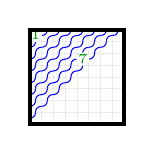
\begin{tikzpicture}[scale=0.15]
  \draw[lightgray, very thin, opacity=0.3] (0,0) -- (8,0);
  \draw[lightgray, very thin, opacity=0.3] (0,0) -- (0,8);
  \draw[lightgray, very thin, opacity=0.3] (0,1) -- (8,1);
  \draw[lightgray, very thin, opacity=0.3] (1,0) -- (1,8);
  \draw[lightgray, very thin, opacity=0.3] (0,2) -- (8,2);
  \draw[lightgray, very thin, opacity=0.3] (2,0) -- (2,8);
  \draw[lightgray, very thin, opacity=0.3] (0,3) -- (8,3);
  \draw[lightgray, very thin, opacity=0.3] (3,0) -- (3,8);
  \draw[lightgray, very thin, opacity=0.3] (0,4) -- (8,4);
  \draw[lightgray, very thin, opacity=0.3] (4,0) -- (4,8);
  \draw[lightgray, very thin, opacity=0.3] (0,5) -- (8,5);
  \draw[lightgray, very thin, opacity=0.3] (5,0) -- (5,8);
  \draw[lightgray, very thin, opacity=0.3] (0,6) -- (8,6);
  \draw[lightgray, very thin, opacity=0.3] (6,0) -- (6,8);
  \draw[lightgray, very thin, opacity=0.3] (0,7) -- (8,7);
  \draw[lightgray, very thin, opacity=0.3] (7,0) -- (7,8);
  \draw[lightgray, very thin, opacity=0.3] (0,8) -- (8,8);
  \draw[lightgray, very thin, opacity=0.3] (8,0) -- (8,8);
  \draw[blue, line width=0.375pt, line cap=round] (0,7.5) -- (1,7.5);
  \draw[blue, line width=0.375pt, line cap=round] (0.5,7) -- (0.5,8);
  \draw[blue, line width=0.375pt] (1,7.5) .. controls (1.3,7.5) and (1.5,7.7) .. (1.5,8);
  \draw[blue, line width=0.375pt] (1.5,7) .. controls (1.5,7.3) and (1.7,7.5) .. (2,7.5);
  \draw[blue, line width=0.375pt] (2,7.5) .. controls (2.3,7.5) and (2.5,7.7) .. (2.5,8);
  \draw[blue, line width=0.375pt] (2.5,7) .. controls (2.5,7.3) and (2.7,7.5) .. (3,7.5);
  \draw[blue, line width=0.375pt] (3,7.5) .. controls (3.3,7.5) and (3.5,7.7) .. (3.5,8);
  \draw[blue, line width=0.375pt] (3.5,7) .. controls (3.5,7.3) and (3.7,7.5) .. (4,7.5);
  \draw[blue, line width=0.375pt] (4,7.5) .. controls (4.3,7.5) and (4.5,7.7) .. (4.5,8);
  \draw[blue, line width=0.375pt] (4.5,7) .. controls (4.5,7.3) and (4.7,7.5) .. (5,7.5);
  \draw[blue, line width=0.375pt] (5,7.5) .. controls (5.3,7.5) and (5.5,7.7) .. (5.5,8);
  \draw[blue, line width=0.375pt] (5.5,7) .. controls (5.5,7.3) and (5.7,7.5) .. (6,7.5);
  \draw[blue, line width=0.375pt] (6,7.5) .. controls (6.3,7.5) and (6.5,7.7) .. (6.5,8);
  \draw[blue, line width=0.375pt] (6.5,7) .. controls (6.5,7.3) and (6.7,7.5) .. (7,7.5);
  \draw[blue, line width=0.375pt] (7,7.5) .. controls (7.3,7.5) and (7.5,7.7) .. (7.5,8);
  \draw[blue, line width=0.375pt] (0,6.5) .. controls (0.3,6.5) and (0.5,6.7) .. (0.5,7);
  \draw[blue, line width=0.375pt] (0.5,6) .. controls (0.5,6.3) and (0.7,6.5) .. (1,6.5);
  \draw[blue, line width=0.375pt] (1,6.5) .. controls (1.3,6.5) and (1.5,6.7) .. (1.5,7);
  \draw[blue, line width=0.375pt] (1.5,6) .. controls (1.5,6.3) and (1.7,6.5) .. (2,6.5);
  \draw[blue, line width=0.375pt] (2,6.5) .. controls (2.3,6.5) and (2.5,6.7) .. (2.5,7);
  \draw[blue, line width=0.375pt] (2.5,6) .. controls (2.5,6.3) and (2.7,6.5) .. (3,6.5);
  \draw[blue, line width=0.375pt] (3,6.5) .. controls (3.3,6.5) and (3.5,6.7) .. (3.5,7);
  \draw[blue, line width=0.375pt] (3.5,6) .. controls (3.5,6.3) and (3.7,6.5) .. (4,6.5);
  \draw[blue, line width=0.375pt] (4,6.5) .. controls (4.3,6.5) and (4.5,6.7) .. (4.5,7);
  \draw[blue, line width=0.375pt] (4.5,6) .. controls (4.5,6.3) and (4.7,6.5) .. (5,6.5);
  \draw[blue, line width=0.375pt] (5,6.5) .. controls (5.3,6.5) and (5.5,6.7) .. (5.5,7);
  \draw[blue, line width=0.375pt] (5.5,6) .. controls (5.5,6.3) and (5.7,6.5) .. (6,6.5);
  \draw[blue, line width=0.375pt] (6,6.5) .. controls (6.3,6.5) and (6.5,6.7) .. (6.5,7);
  \draw[blue, line width=0.375pt] (0,5.5) .. controls (0.3,5.5) and (0.5,5.7) .. (0.5,6);
  \draw[blue, line width=0.375pt] (0.5,5) .. controls (0.5,5.3) and (0.7,5.5) .. (1,5.5);
  \draw[blue, line width=0.375pt] (1,5.5) .. controls (1.3,5.5) and (1.5,5.7) .. (1.5,6);
  \draw[blue, line width=0.375pt] (1.5,5) .. controls (1.5,5.3) and (1.7,5.5) .. (2,5.5);
  \draw[blue, line width=0.375pt] (2,5.5) .. controls (2.3,5.5) and (2.5,5.7) .. (2.5,6);
  \draw[blue, line width=0.375pt] (2.5,5) .. controls (2.5,5.3) and (2.7,5.5) .. (3,5.5);
  \draw[blue, line width=0.375pt] (3,5.5) .. controls (3.3,5.5) and (3.5,5.7) .. (3.5,6);
  \draw[blue, line width=0.375pt] (3.5,5) .. controls (3.5,5.3) and (3.7,5.5) .. (4,5.5);
  \draw[blue, line width=0.375pt, line cap=round] (4,5.5) -- (5,5.5);
  \draw[blue, line width=0.375pt, line cap=round] (4.5,5) -- (4.5,6);
  \draw[blue, line width=0.375pt] (5,5.5) .. controls (5.3,5.5) and (5.5,5.7) .. (5.5,6);
  \draw[blue, line width=0.375pt] (0,4.5) .. controls (0.3,4.5) and (0.5,4.7) .. (0.5,5);
  \draw[blue, line width=0.375pt] (0.5,4) .. controls (0.5,4.3) and (0.7,4.5) .. (1,4.5);
  \draw[blue, line width=0.375pt] (1,4.5) .. controls (1.3,4.5) and (1.5,4.7) .. (1.5,5);
  \draw[blue, line width=0.375pt] (1.5,4) .. controls (1.5,4.3) and (1.7,4.5) .. (2,4.5);
  \draw[blue, line width=0.375pt] (2,4.5) .. controls (2.3,4.5) and (2.5,4.7) .. (2.5,5);
  \draw[blue, line width=0.375pt] (2.5,4) .. controls (2.5,4.3) and (2.7,4.5) .. (3,4.5);
  \draw[blue, line width=0.375pt] (3,4.5) .. controls (3.3,4.5) and (3.5,4.7) .. (3.5,5);
  \draw[blue, line width=0.375pt] (3.5,4) .. controls (3.5,4.3) and (3.7,4.5) .. (4,4.5);
  \draw[blue, line width=0.375pt] (4,4.5) .. controls (4.3,4.5) and (4.5,4.7) .. (4.5,5);
  \draw[blue, line width=0.375pt] (0,3.5) .. controls (0.3,3.5) and (0.5,3.7) .. (0.5,4);
  \draw[blue, line width=0.375pt] (0.5,3) .. controls (0.5,3.3) and (0.7,3.5) .. (1,3.5);
  \draw[blue, line width=0.375pt] (1,3.5) .. controls (1.3,3.5) and (1.5,3.7) .. (1.5,4);
  \draw[blue, line width=0.375pt] (1.5,3) .. controls (1.5,3.3) and (1.7,3.5) .. (2,3.5);
  \draw[blue, line width=0.375pt] (2,3.5) .. controls (2.3,3.5) and (2.5,3.7) .. (2.5,4);
  \draw[blue, line width=0.375pt] (2.5,3) .. controls (2.5,3.3) and (2.7,3.5) .. (3,3.5);
  \draw[blue, line width=0.375pt] (3,3.5) .. controls (3.3,3.5) and (3.5,3.7) .. (3.5,4);
  \draw[blue, line width=0.375pt] (0,2.5) .. controls (0.3,2.5) and (0.5,2.7) .. (0.5,3);
  \draw[blue, line width=0.375pt] (0.5,2) .. controls (0.5,2.3) and (0.7,2.5) .. (1,2.5);
  \draw[blue, line width=0.375pt] (1,2.5) .. controls (1.3,2.5) and (1.5,2.7) .. (1.5,3);
  \draw[blue, line width=0.375pt] (1.5,2) .. controls (1.5,2.3) and (1.7,2.5) .. (2,2.5);
  \draw[blue, line width=0.375pt] (2,2.5) .. controls (2.3,2.5) and (2.5,2.7) .. (2.5,3);
  \draw[blue, line width=0.375pt] (0,1.5) .. controls (0.3,1.5) and (0.5,1.7) .. (0.5,2);
  \draw[blue, line width=0.375pt] (0.5,1) .. controls (0.5,1.3) and (0.7,1.5) .. (1,1.5);
  \draw[blue, line width=0.375pt] (1,1.5) .. controls (1.3,1.5) and (1.5,1.7) .. (1.5,2);
  \draw[blue, line width=0.375pt] (0,0.5) .. controls (0.3,0.5) and (0.5,0.7) .. (0.5,1);
  \node[font=\fontsize{3}{3}\selectfont, text=green!60!black, fill=white, inner sep=0pt, circle] at (0.5,7.5) {1};
  \node[font=\fontsize{3}{3}\selectfont, text=green!60!black, fill=white, inner sep=0pt, circle] at (4.5,5.5) {7};
  \draw[black, line width=1.4pt] (0,0) rectangle (8,8);
\end{tikzpicture}
  \end{minipage}

  \vspace{0.3em}
  $rc \star rc_2 =$
  \begin{minipage}{0.22\textwidth}\centering
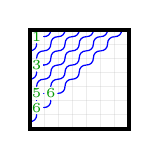
\begin{tikzpicture}[scale=0.18]
  \draw[lightgray, very thin, opacity=0.3] (0,0) -- (7,0);
  \draw[lightgray, very thin, opacity=0.3] (0,0) -- (0,7);
  \draw[lightgray, very thin, opacity=0.3] (0,1) -- (7,1);
  \draw[lightgray, very thin, opacity=0.3] (1,0) -- (1,7);
  \draw[lightgray, very thin, opacity=0.3] (0,2) -- (7,2);
  \draw[lightgray, very thin, opacity=0.3] (2,0) -- (2,7);
  \draw[lightgray, very thin, opacity=0.3] (0,3) -- (7,3);
  \draw[lightgray, very thin, opacity=0.3] (3,0) -- (3,7);
  \draw[lightgray, very thin, opacity=0.3] (0,4) -- (7,4);
  \draw[lightgray, very thin, opacity=0.3] (4,0) -- (4,7);
  \draw[lightgray, very thin, opacity=0.3] (0,5) -- (7,5);
  \draw[lightgray, very thin, opacity=0.3] (5,0) -- (5,7);
  \draw[lightgray, very thin, opacity=0.3] (0,6) -- (7,6);
  \draw[lightgray, very thin, opacity=0.3] (6,0) -- (6,7);
  \draw[lightgray, very thin, opacity=0.3] (0,7) -- (7,7);
  \draw[lightgray, very thin, opacity=0.3] (7,0) -- (7,7);
  \draw[blue, line width=0.44999999999999996pt, line cap=round] (0,6.5) -- (1,6.5);
  \draw[blue, line width=0.44999999999999996pt, line cap=round] (0.5,6) -- (0.5,7);
  \draw[blue, line width=0.44999999999999996pt] (1,6.5) .. controls (1.3,6.5) and (1.5,6.7) .. (1.5,7);
  \draw[blue, line width=0.44999999999999996pt] (1.5,6) .. controls (1.5,6.3) and (1.7,6.5) .. (2,6.5);
  \draw[blue, line width=0.44999999999999996pt] (2,6.5) .. controls (2.3,6.5) and (2.5,6.7) .. (2.5,7);
  \draw[blue, line width=0.44999999999999996pt] (2.5,6) .. controls (2.5,6.3) and (2.7,6.5) .. (3,6.5);
  \draw[blue, line width=0.44999999999999996pt] (3,6.5) .. controls (3.3,6.5) and (3.5,6.7) .. (3.5,7);
  \draw[blue, line width=0.44999999999999996pt] (3.5,6) .. controls (3.5,6.3) and (3.7,6.5) .. (4,6.5);
  \draw[blue, line width=0.44999999999999996pt] (4,6.5) .. controls (4.3,6.5) and (4.5,6.7) .. (4.5,7);
  \draw[blue, line width=0.44999999999999996pt] (4.5,6) .. controls (4.5,6.3) and (4.7,6.5) .. (5,6.5);
  \draw[blue, line width=0.44999999999999996pt] (5,6.5) .. controls (5.3,6.5) and (5.5,6.7) .. (5.5,7);
  \draw[blue, line width=0.44999999999999996pt] (5.5,6) .. controls (5.5,6.3) and (5.7,6.5) .. (6,6.5);
  \draw[blue, line width=0.44999999999999996pt] (6,6.5) .. controls (6.3,6.5) and (6.5,6.7) .. (6.5,7);
  \draw[blue, line width=0.44999999999999996pt] (0,5.5) .. controls (0.3,5.5) and (0.5,5.7) .. (0.5,6);
  \draw[blue, line width=0.44999999999999996pt] (0.5,5) .. controls (0.5,5.3) and (0.7,5.5) .. (1,5.5);
  \draw[blue, line width=0.44999999999999996pt] (1,5.5) .. controls (1.3,5.5) and (1.5,5.7) .. (1.5,6);
  \draw[blue, line width=0.44999999999999996pt] (1.5,5) .. controls (1.5,5.3) and (1.7,5.5) .. (2,5.5);
  \draw[blue, line width=0.44999999999999996pt] (2,5.5) .. controls (2.3,5.5) and (2.5,5.7) .. (2.5,6);
  \draw[blue, line width=0.44999999999999996pt] (2.5,5) .. controls (2.5,5.3) and (2.7,5.5) .. (3,5.5);
  \draw[blue, line width=0.44999999999999996pt] (3,5.5) .. controls (3.3,5.5) and (3.5,5.7) .. (3.5,6);
  \draw[blue, line width=0.44999999999999996pt] (3.5,5) .. controls (3.5,5.3) and (3.7,5.5) .. (4,5.5);
  \draw[blue, line width=0.44999999999999996pt] (4,5.5) .. controls (4.3,5.5) and (4.5,5.7) .. (4.5,6);
  \draw[blue, line width=0.44999999999999996pt] (4.5,5) .. controls (4.5,5.3) and (4.7,5.5) .. (5,5.5);
  \draw[blue, line width=0.44999999999999996pt] (5,5.5) .. controls (5.3,5.5) and (5.5,5.7) .. (5.5,6);
  \draw[blue, line width=0.44999999999999996pt, line cap=round] (0,4.5) -- (1,4.5);
  \draw[blue, line width=0.44999999999999996pt, line cap=round] (0.5,4) -- (0.5,5);
  \draw[blue, line width=0.44999999999999996pt] (1,4.5) .. controls (1.3,4.5) and (1.5,4.7) .. (1.5,5);
  \draw[blue, line width=0.44999999999999996pt] (1.5,4) .. controls (1.5,4.3) and (1.7,4.5) .. (2,4.5);
  \draw[blue, line width=0.44999999999999996pt] (2,4.5) .. controls (2.3,4.5) and (2.5,4.7) .. (2.5,5);
  \draw[blue, line width=0.44999999999999996pt] (2.5,4) .. controls (2.5,4.3) and (2.7,4.5) .. (3,4.5);
  \draw[blue, line width=0.44999999999999996pt] (3,4.5) .. controls (3.3,4.5) and (3.5,4.7) .. (3.5,5);
  \draw[blue, line width=0.44999999999999996pt] (3.5,4) .. controls (3.5,4.3) and (3.7,4.5) .. (4,4.5);
  \draw[blue, line width=0.44999999999999996pt] (4,4.5) .. controls (4.3,4.5) and (4.5,4.7) .. (4.5,5);
  \draw[blue, line width=0.44999999999999996pt] (0,3.5) .. controls (0.3,3.5) and (0.5,3.7) .. (0.5,4);
  \draw[blue, line width=0.44999999999999996pt] (0.5,3) .. controls (0.5,3.3) and (0.7,3.5) .. (1,3.5);
  \draw[blue, line width=0.44999999999999996pt] (1,3.5) .. controls (1.3,3.5) and (1.5,3.7) .. (1.5,4);
  \draw[blue, line width=0.44999999999999996pt] (1.5,3) .. controls (1.5,3.3) and (1.7,3.5) .. (2,3.5);
  \draw[blue, line width=0.44999999999999996pt] (2,3.5) .. controls (2.3,3.5) and (2.5,3.7) .. (2.5,4);
  \draw[blue, line width=0.44999999999999996pt] (2.5,3) .. controls (2.5,3.3) and (2.7,3.5) .. (3,3.5);
  \draw[blue, line width=0.44999999999999996pt] (3,3.5) .. controls (3.3,3.5) and (3.5,3.7) .. (3.5,4);
  \draw[blue, line width=0.44999999999999996pt, line cap=round] (0,2.5) -- (1,2.5);
  \draw[blue, line width=0.44999999999999996pt, line cap=round] (0.5,2) -- (0.5,3);
  \draw[blue, line width=0.44999999999999996pt, line cap=round] (1,2.5) -- (2,2.5);
  \draw[blue, line width=0.44999999999999996pt, line cap=round] (1.5,2) -- (1.5,3);
  \draw[blue, line width=0.44999999999999996pt] (2,2.5) .. controls (2.3,2.5) and (2.5,2.7) .. (2.5,3);
  \draw[blue, line width=0.44999999999999996pt, line cap=round] (0,1.5) -- (1,1.5);
  \draw[blue, line width=0.44999999999999996pt, line cap=round] (0.5,1) -- (0.5,2);
  \draw[blue, line width=0.44999999999999996pt] (1,1.5) .. controls (1.3,1.5) and (1.5,1.7) .. (1.5,2);
  \draw[blue, line width=0.44999999999999996pt] (0,0.5) .. controls (0.3,0.5) and (0.5,0.7) .. (0.5,1);
  \node[font=\fontsize{3}{3}\selectfont, text=green!60!black, fill=white, inner sep=0pt, circle] at (0.5,4.5) {3};
  \node[font=\fontsize{3}{3}\selectfont, text=green!60!black, fill=white, inner sep=0pt, circle] at (0.5,1.5) {6};
  \node[font=\fontsize{3}{3}\selectfont, text=green!60!black, fill=white, inner sep=0pt, circle] at (0.5,6.5) {1};
  \node[font=\fontsize{3}{3}\selectfont, text=green!60!black, fill=white, inner sep=0pt, circle] at (0.5,2.5) {5};
  \node[font=\fontsize{3}{3}\selectfont, text=green!60!black, fill=white, inner sep=0pt, circle] at (1.5,2.5) {6};
  \draw[black, line width=1.4pt] (0,0) rectangle (7,7);
\end{tikzpicture}
  \end{minipage}
  $+$
  \begin{minipage}{0.22\textwidth}\centering
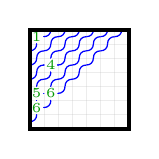
\begin{tikzpicture}[scale=0.18]
  \draw[lightgray, very thin, opacity=0.3] (0,0) -- (7,0);
  \draw[lightgray, very thin, opacity=0.3] (0,0) -- (0,7);
  \draw[lightgray, very thin, opacity=0.3] (0,1) -- (7,1);
  \draw[lightgray, very thin, opacity=0.3] (1,0) -- (1,7);
  \draw[lightgray, very thin, opacity=0.3] (0,2) -- (7,2);
  \draw[lightgray, very thin, opacity=0.3] (2,0) -- (2,7);
  \draw[lightgray, very thin, opacity=0.3] (0,3) -- (7,3);
  \draw[lightgray, very thin, opacity=0.3] (3,0) -- (3,7);
  \draw[lightgray, very thin, opacity=0.3] (0,4) -- (7,4);
  \draw[lightgray, very thin, opacity=0.3] (4,0) -- (4,7);
  \draw[lightgray, very thin, opacity=0.3] (0,5) -- (7,5);
  \draw[lightgray, very thin, opacity=0.3] (5,0) -- (5,7);
  \draw[lightgray, very thin, opacity=0.3] (0,6) -- (7,6);
  \draw[lightgray, very thin, opacity=0.3] (6,0) -- (6,7);
  \draw[lightgray, very thin, opacity=0.3] (0,7) -- (7,7);
  \draw[lightgray, very thin, opacity=0.3] (7,0) -- (7,7);
  \draw[blue, line width=0.44999999999999996pt, line cap=round] (0,6.5) -- (1,6.5);
  \draw[blue, line width=0.44999999999999996pt, line cap=round] (0.5,6) -- (0.5,7);
  \draw[blue, line width=0.44999999999999996pt] (1,6.5) .. controls (1.3,6.5) and (1.5,6.7) .. (1.5,7);
  \draw[blue, line width=0.44999999999999996pt] (1.5,6) .. controls (1.5,6.3) and (1.7,6.5) .. (2,6.5);
  \draw[blue, line width=0.44999999999999996pt] (2,6.5) .. controls (2.3,6.5) and (2.5,6.7) .. (2.5,7);
  \draw[blue, line width=0.44999999999999996pt] (2.5,6) .. controls (2.5,6.3) and (2.7,6.5) .. (3,6.5);
  \draw[blue, line width=0.44999999999999996pt] (3,6.5) .. controls (3.3,6.5) and (3.5,6.7) .. (3.5,7);
  \draw[blue, line width=0.44999999999999996pt] (3.5,6) .. controls (3.5,6.3) and (3.7,6.5) .. (4,6.5);
  \draw[blue, line width=0.44999999999999996pt] (4,6.5) .. controls (4.3,6.5) and (4.5,6.7) .. (4.5,7);
  \draw[blue, line width=0.44999999999999996pt] (4.5,6) .. controls (4.5,6.3) and (4.7,6.5) .. (5,6.5);
  \draw[blue, line width=0.44999999999999996pt] (5,6.5) .. controls (5.3,6.5) and (5.5,6.7) .. (5.5,7);
  \draw[blue, line width=0.44999999999999996pt] (5.5,6) .. controls (5.5,6.3) and (5.7,6.5) .. (6,6.5);
  \draw[blue, line width=0.44999999999999996pt] (6,6.5) .. controls (6.3,6.5) and (6.5,6.7) .. (6.5,7);
  \draw[blue, line width=0.44999999999999996pt] (0,5.5) .. controls (0.3,5.5) and (0.5,5.7) .. (0.5,6);
  \draw[blue, line width=0.44999999999999996pt] (0.5,5) .. controls (0.5,5.3) and (0.7,5.5) .. (1,5.5);
  \draw[blue, line width=0.44999999999999996pt] (1,5.5) .. controls (1.3,5.5) and (1.5,5.7) .. (1.5,6);
  \draw[blue, line width=0.44999999999999996pt] (1.5,5) .. controls (1.5,5.3) and (1.7,5.5) .. (2,5.5);
  \draw[blue, line width=0.44999999999999996pt] (2,5.5) .. controls (2.3,5.5) and (2.5,5.7) .. (2.5,6);
  \draw[blue, line width=0.44999999999999996pt] (2.5,5) .. controls (2.5,5.3) and (2.7,5.5) .. (3,5.5);
  \draw[blue, line width=0.44999999999999996pt] (3,5.5) .. controls (3.3,5.5) and (3.5,5.7) .. (3.5,6);
  \draw[blue, line width=0.44999999999999996pt] (3.5,5) .. controls (3.5,5.3) and (3.7,5.5) .. (4,5.5);
  \draw[blue, line width=0.44999999999999996pt] (4,5.5) .. controls (4.3,5.5) and (4.5,5.7) .. (4.5,6);
  \draw[blue, line width=0.44999999999999996pt] (4.5,5) .. controls (4.5,5.3) and (4.7,5.5) .. (5,5.5);
  \draw[blue, line width=0.44999999999999996pt] (5,5.5) .. controls (5.3,5.5) and (5.5,5.7) .. (5.5,6);
  \draw[blue, line width=0.44999999999999996pt] (0,4.5) .. controls (0.3,4.5) and (0.5,4.7) .. (0.5,5);
  \draw[blue, line width=0.44999999999999996pt] (0.5,4) .. controls (0.5,4.3) and (0.7,4.5) .. (1,4.5);
  \draw[blue, line width=0.44999999999999996pt, line cap=round] (1,4.5) -- (2,4.5);
  \draw[blue, line width=0.44999999999999996pt, line cap=round] (1.5,4) -- (1.5,5);
  \draw[blue, line width=0.44999999999999996pt] (2,4.5) .. controls (2.3,4.5) and (2.5,4.7) .. (2.5,5);
  \draw[blue, line width=0.44999999999999996pt] (2.5,4) .. controls (2.5,4.3) and (2.7,4.5) .. (3,4.5);
  \draw[blue, line width=0.44999999999999996pt] (3,4.5) .. controls (3.3,4.5) and (3.5,4.7) .. (3.5,5);
  \draw[blue, line width=0.44999999999999996pt] (3.5,4) .. controls (3.5,4.3) and (3.7,4.5) .. (4,4.5);
  \draw[blue, line width=0.44999999999999996pt] (4,4.5) .. controls (4.3,4.5) and (4.5,4.7) .. (4.5,5);
  \draw[blue, line width=0.44999999999999996pt] (0,3.5) .. controls (0.3,3.5) and (0.5,3.7) .. (0.5,4);
  \draw[blue, line width=0.44999999999999996pt] (0.5,3) .. controls (0.5,3.3) and (0.7,3.5) .. (1,3.5);
  \draw[blue, line width=0.44999999999999996pt] (1,3.5) .. controls (1.3,3.5) and (1.5,3.7) .. (1.5,4);
  \draw[blue, line width=0.44999999999999996pt] (1.5,3) .. controls (1.5,3.3) and (1.7,3.5) .. (2,3.5);
  \draw[blue, line width=0.44999999999999996pt] (2,3.5) .. controls (2.3,3.5) and (2.5,3.7) .. (2.5,4);
  \draw[blue, line width=0.44999999999999996pt] (2.5,3) .. controls (2.5,3.3) and (2.7,3.5) .. (3,3.5);
  \draw[blue, line width=0.44999999999999996pt] (3,3.5) .. controls (3.3,3.5) and (3.5,3.7) .. (3.5,4);
  \draw[blue, line width=0.44999999999999996pt, line cap=round] (0,2.5) -- (1,2.5);
  \draw[blue, line width=0.44999999999999996pt, line cap=round] (0.5,2) -- (0.5,3);
  \draw[blue, line width=0.44999999999999996pt, line cap=round] (1,2.5) -- (2,2.5);
  \draw[blue, line width=0.44999999999999996pt, line cap=round] (1.5,2) -- (1.5,3);
  \draw[blue, line width=0.44999999999999996pt] (2,2.5) .. controls (2.3,2.5) and (2.5,2.7) .. (2.5,3);
  \draw[blue, line width=0.44999999999999996pt, line cap=round] (0,1.5) -- (1,1.5);
  \draw[blue, line width=0.44999999999999996pt, line cap=round] (0.5,1) -- (0.5,2);
  \draw[blue, line width=0.44999999999999996pt] (1,1.5) .. controls (1.3,1.5) and (1.5,1.7) .. (1.5,2);
  \draw[blue, line width=0.44999999999999996pt] (0,0.5) .. controls (0.3,0.5) and (0.5,0.7) .. (0.5,1);
  \node[font=\fontsize{3}{3}\selectfont, text=green!60!black, fill=white, inner sep=0pt, circle] at (0.5,1.5) {6};
  \node[font=\fontsize{3}{3}\selectfont, text=green!60!black, fill=white, inner sep=0pt, circle] at (0.5,6.5) {1};
  \node[font=\fontsize{3}{3}\selectfont, text=green!60!black, fill=white, inner sep=0pt, circle] at (0.5,2.5) {5};
  \node[font=\fontsize{3}{3}\selectfont, text=green!60!black, fill=white, inner sep=0pt, circle] at (1.5,4.5) {4};
  \node[font=\fontsize{3}{3}\selectfont, text=green!60!black, fill=white, inner sep=0pt, circle] at (1.5,2.5) {6};
  \draw[black, line width=1.4pt] (0,0) rectangle (7,7);
\end{tikzpicture}
  \end{minipage}
  $+$
  \begin{minipage}{0.22\textwidth}\centering
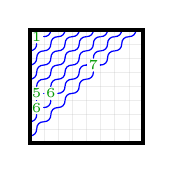
\begin{tikzpicture}[scale=0.18]
  \draw[lightgray, very thin, opacity=0.3] (0,0) -- (8,0);
  \draw[lightgray, very thin, opacity=0.3] (0,0) -- (0,8);
  \draw[lightgray, very thin, opacity=0.3] (0,1) -- (8,1);
  \draw[lightgray, very thin, opacity=0.3] (1,0) -- (1,8);
  \draw[lightgray, very thin, opacity=0.3] (0,2) -- (8,2);
  \draw[lightgray, very thin, opacity=0.3] (2,0) -- (2,8);
  \draw[lightgray, very thin, opacity=0.3] (0,3) -- (8,3);
  \draw[lightgray, very thin, opacity=0.3] (3,0) -- (3,8);
  \draw[lightgray, very thin, opacity=0.3] (0,4) -- (8,4);
  \draw[lightgray, very thin, opacity=0.3] (4,0) -- (4,8);
  \draw[lightgray, very thin, opacity=0.3] (0,5) -- (8,5);
  \draw[lightgray, very thin, opacity=0.3] (5,0) -- (5,8);
  \draw[lightgray, very thin, opacity=0.3] (0,6) -- (8,6);
  \draw[lightgray, very thin, opacity=0.3] (6,0) -- (6,8);
  \draw[lightgray, very thin, opacity=0.3] (0,7) -- (8,7);
  \draw[lightgray, very thin, opacity=0.3] (7,0) -- (7,8);
  \draw[lightgray, very thin, opacity=0.3] (0,8) -- (8,8);
  \draw[lightgray, very thin, opacity=0.3] (8,0) -- (8,8);
  \draw[blue, line width=0.44999999999999996pt, line cap=round] (0,7.5) -- (1,7.5);
  \draw[blue, line width=0.44999999999999996pt, line cap=round] (0.5,7) -- (0.5,8);
  \draw[blue, line width=0.44999999999999996pt] (1,7.5) .. controls (1.3,7.5) and (1.5,7.7) .. (1.5,8);
  \draw[blue, line width=0.44999999999999996pt] (1.5,7) .. controls (1.5,7.3) and (1.7,7.5) .. (2,7.5);
  \draw[blue, line width=0.44999999999999996pt] (2,7.5) .. controls (2.3,7.5) and (2.5,7.7) .. (2.5,8);
  \draw[blue, line width=0.44999999999999996pt] (2.5,7) .. controls (2.5,7.3) and (2.7,7.5) .. (3,7.5);
  \draw[blue, line width=0.44999999999999996pt] (3,7.5) .. controls (3.3,7.5) and (3.5,7.7) .. (3.5,8);
  \draw[blue, line width=0.44999999999999996pt] (3.5,7) .. controls (3.5,7.3) and (3.7,7.5) .. (4,7.5);
  \draw[blue, line width=0.44999999999999996pt] (4,7.5) .. controls (4.3,7.5) and (4.5,7.7) .. (4.5,8);
  \draw[blue, line width=0.44999999999999996pt] (4.5,7) .. controls (4.5,7.3) and (4.7,7.5) .. (5,7.5);
  \draw[blue, line width=0.44999999999999996pt] (5,7.5) .. controls (5.3,7.5) and (5.5,7.7) .. (5.5,8);
  \draw[blue, line width=0.44999999999999996pt] (5.5,7) .. controls (5.5,7.3) and (5.7,7.5) .. (6,7.5);
  \draw[blue, line width=0.44999999999999996pt] (6,7.5) .. controls (6.3,7.5) and (6.5,7.7) .. (6.5,8);
  \draw[blue, line width=0.44999999999999996pt] (6.5,7) .. controls (6.5,7.3) and (6.7,7.5) .. (7,7.5);
  \draw[blue, line width=0.44999999999999996pt] (7,7.5) .. controls (7.3,7.5) and (7.5,7.7) .. (7.5,8);
  \draw[blue, line width=0.44999999999999996pt] (0,6.5) .. controls (0.3,6.5) and (0.5,6.7) .. (0.5,7);
  \draw[blue, line width=0.44999999999999996pt] (0.5,6) .. controls (0.5,6.3) and (0.7,6.5) .. (1,6.5);
  \draw[blue, line width=0.44999999999999996pt] (1,6.5) .. controls (1.3,6.5) and (1.5,6.7) .. (1.5,7);
  \draw[blue, line width=0.44999999999999996pt] (1.5,6) .. controls (1.5,6.3) and (1.7,6.5) .. (2,6.5);
  \draw[blue, line width=0.44999999999999996pt] (2,6.5) .. controls (2.3,6.5) and (2.5,6.7) .. (2.5,7);
  \draw[blue, line width=0.44999999999999996pt] (2.5,6) .. controls (2.5,6.3) and (2.7,6.5) .. (3,6.5);
  \draw[blue, line width=0.44999999999999996pt] (3,6.5) .. controls (3.3,6.5) and (3.5,6.7) .. (3.5,7);
  \draw[blue, line width=0.44999999999999996pt] (3.5,6) .. controls (3.5,6.3) and (3.7,6.5) .. (4,6.5);
  \draw[blue, line width=0.44999999999999996pt] (4,6.5) .. controls (4.3,6.5) and (4.5,6.7) .. (4.5,7);
  \draw[blue, line width=0.44999999999999996pt] (4.5,6) .. controls (4.5,6.3) and (4.7,6.5) .. (5,6.5);
  \draw[blue, line width=0.44999999999999996pt] (5,6.5) .. controls (5.3,6.5) and (5.5,6.7) .. (5.5,7);
  \draw[blue, line width=0.44999999999999996pt] (5.5,6) .. controls (5.5,6.3) and (5.7,6.5) .. (6,6.5);
  \draw[blue, line width=0.44999999999999996pt] (6,6.5) .. controls (6.3,6.5) and (6.5,6.7) .. (6.5,7);
  \draw[blue, line width=0.44999999999999996pt] (0,5.5) .. controls (0.3,5.5) and (0.5,5.7) .. (0.5,6);
  \draw[blue, line width=0.44999999999999996pt] (0.5,5) .. controls (0.5,5.3) and (0.7,5.5) .. (1,5.5);
  \draw[blue, line width=0.44999999999999996pt] (1,5.5) .. controls (1.3,5.5) and (1.5,5.7) .. (1.5,6);
  \draw[blue, line width=0.44999999999999996pt] (1.5,5) .. controls (1.5,5.3) and (1.7,5.5) .. (2,5.5);
  \draw[blue, line width=0.44999999999999996pt] (2,5.5) .. controls (2.3,5.5) and (2.5,5.7) .. (2.5,6);
  \draw[blue, line width=0.44999999999999996pt] (2.5,5) .. controls (2.5,5.3) and (2.7,5.5) .. (3,5.5);
  \draw[blue, line width=0.44999999999999996pt] (3,5.5) .. controls (3.3,5.5) and (3.5,5.7) .. (3.5,6);
  \draw[blue, line width=0.44999999999999996pt] (3.5,5) .. controls (3.5,5.3) and (3.7,5.5) .. (4,5.5);
  \draw[blue, line width=0.44999999999999996pt, line cap=round] (4,5.5) -- (5,5.5);
  \draw[blue, line width=0.44999999999999996pt, line cap=round] (4.5,5) -- (4.5,6);
  \draw[blue, line width=0.44999999999999996pt] (5,5.5) .. controls (5.3,5.5) and (5.5,5.7) .. (5.5,6);
  \draw[blue, line width=0.44999999999999996pt] (0,4.5) .. controls (0.3,4.5) and (0.5,4.7) .. (0.5,5);
  \draw[blue, line width=0.44999999999999996pt] (0.5,4) .. controls (0.5,4.3) and (0.7,4.5) .. (1,4.5);
  \draw[blue, line width=0.44999999999999996pt] (1,4.5) .. controls (1.3,4.5) and (1.5,4.7) .. (1.5,5);
  \draw[blue, line width=0.44999999999999996pt] (1.5,4) .. controls (1.5,4.3) and (1.7,4.5) .. (2,4.5);
  \draw[blue, line width=0.44999999999999996pt] (2,4.5) .. controls (2.3,4.5) and (2.5,4.7) .. (2.5,5);
  \draw[blue, line width=0.44999999999999996pt] (2.5,4) .. controls (2.5,4.3) and (2.7,4.5) .. (3,4.5);
  \draw[blue, line width=0.44999999999999996pt] (3,4.5) .. controls (3.3,4.5) and (3.5,4.7) .. (3.5,5);
  \draw[blue, line width=0.44999999999999996pt] (3.5,4) .. controls (3.5,4.3) and (3.7,4.5) .. (4,4.5);
  \draw[blue, line width=0.44999999999999996pt] (4,4.5) .. controls (4.3,4.5) and (4.5,4.7) .. (4.5,5);
  \draw[blue, line width=0.44999999999999996pt, line cap=round] (0,3.5) -- (1,3.5);
  \draw[blue, line width=0.44999999999999996pt, line cap=round] (0.5,3) -- (0.5,4);
  \draw[blue, line width=0.44999999999999996pt, line cap=round] (1,3.5) -- (2,3.5);
  \draw[blue, line width=0.44999999999999996pt, line cap=round] (1.5,3) -- (1.5,4);
  \draw[blue, line width=0.44999999999999996pt] (2,3.5) .. controls (2.3,3.5) and (2.5,3.7) .. (2.5,4);
  \draw[blue, line width=0.44999999999999996pt] (2.5,3) .. controls (2.5,3.3) and (2.7,3.5) .. (3,3.5);
  \draw[blue, line width=0.44999999999999996pt] (3,3.5) .. controls (3.3,3.5) and (3.5,3.7) .. (3.5,4);
  \draw[blue, line width=0.44999999999999996pt, line cap=round] (0,2.5) -- (1,2.5);
  \draw[blue, line width=0.44999999999999996pt, line cap=round] (0.5,2) -- (0.5,3);
  \draw[blue, line width=0.44999999999999996pt] (1,2.5) .. controls (1.3,2.5) and (1.5,2.7) .. (1.5,3);
  \draw[blue, line width=0.44999999999999996pt] (1.5,2) .. controls (1.5,2.3) and (1.7,2.5) .. (2,2.5);
  \draw[blue, line width=0.44999999999999996pt] (2,2.5) .. controls (2.3,2.5) and (2.5,2.7) .. (2.5,3);
  \draw[blue, line width=0.44999999999999996pt] (0,1.5) .. controls (0.3,1.5) and (0.5,1.7) .. (0.5,2);
  \draw[blue, line width=0.44999999999999996pt] (0.5,1) .. controls (0.5,1.3) and (0.7,1.5) .. (1,1.5);
  \draw[blue, line width=0.44999999999999996pt] (1,1.5) .. controls (1.3,1.5) and (1.5,1.7) .. (1.5,2);
  \draw[blue, line width=0.44999999999999996pt] (0,0.5) .. controls (0.3,0.5) and (0.5,0.7) .. (0.5,1);
  \node[font=\fontsize{3}{3}\selectfont, text=green!60!black, fill=white, inner sep=0pt, circle] at (0.5,2.5) {6};
  \node[font=\fontsize{3}{3}\selectfont, text=green!60!black, fill=white, inner sep=0pt, circle] at (0.5,7.5) {1};
  \node[font=\fontsize{3}{3}\selectfont, text=green!60!black, fill=white, inner sep=0pt, circle] at (0.5,3.5) {5};
  \node[font=\fontsize{3}{3}\selectfont, text=green!60!black, fill=white, inner sep=0pt, circle] at (4.5,5.5) {7};
  \node[font=\fontsize{3}{3}\selectfont, text=green!60!black, fill=white, inner sep=0pt, circle] at (1.5,3.5) {6};
  \draw[black, line width=1.4pt] (0,0) rectangle (8,8);
\end{tikzpicture}
  \end{minipage}
\end{frame}




\begin{frame}{Pipe dream ring as a lift of $\dcoma$}
There are two surjective linear maps from the pipe dream ring $\RC$ to the dual algebra $\dcoma$:
\[
\pi_{\mathrm{Sch}}:\RC\twoheadrightarrow \dcoma,\qquad
\pi_{\mathrm{Sch}}(G)=\Sch{\mathrm{perm}(G)}^{(n)},
\]
\[
\pi_{\mathrm{wt}}:\RC\twoheadrightarrow \dcoma,\qquad
\pi_{\mathrm{wt}}(G)=\wb{\mathrm{wt}(G)}.
\]
By virtue of the fact that $\dcoma$ is free, there is a section $\iota:\dcoma\hookrightarrow \RC$ of $\pi_{\mathrm{wt}}$ that sends $\wb{i}$ for an integer $i$ to the unique pipe dream $r_i$ with $\mathrm{wt}(r_i)=(i)$. It turns out that these are all ring homomorphisms and $\iota$ is also a section of $\pi_{\mathrm{Sch}}$.
\begin{theorem}[S, 2026+]
We have that $\pi_{\mathrm{Sch}}$ and $\pi_{\mathrm{wt}}$ are surjective ring homomorphisms to $\dcoma$ and $\iota$ is an injective ring homomorphism from $\dcoma$ to $\RC$ such that
$$\pi_{\mathrm{Sch}} \circ \iota = \pi_{\mathrm{wt}} \circ \iota = \mathrm{id}_{\dcoma}.$$
\end{theorem}

% Hence pipe dreams are a bijective dictionary between the Schubert basis and the word basis that respects the algebra structure.
%Under the basis identification in $\dcoma$, these describe the same surjective ring homomorphism (Schubert coordinates versus word coordinates).
\end{frame}

% \begin{frame}{Direct sum decomposition of $\mathcal{R}$}
% Consider the two-sided ideal $I$ of $\mathcal{R}$ generated by $R_1 - R_2$, where $w(R_1) = w(R_2)$. Then $\mathcal{R} = I \oplus \iota(\dcoma)$ as a vector space, and the projection map $\pi_{\mathrm{Sch}}$ is the projection onto the second factor. In particular, $\iota(\dcoma)$ is a subalgebra of $\mathcal{R}$ isomorphic to $\dcoma$.

% \begin{theorem}
% If $\{\mathfrak{A}_\alpha\}$ is a Schubert positive homogeneous basis of $\dcoma$, then there is a unique representation
% $$\iota(\mathfrak{A}_\alpha) = \sum_{w\in P_\alpha,R'\in \RC(w)}a_{\alpha}^{R'}R' + \sum_{R\in\RC\setminus I_\alpha} c_\alpha^R R$$
% where $c_\alpha^R \geq 0$ for all $R$. 
% % In this situation, choose $w$ such that $c_\alpha^R=1$ for some $R\in \RC(w)$. Then the dual basis $\{\mathcal{A}_\alpha\}$ in $\coma$ satisfies
% % $$\mathcal{A}_\alpha = \sum_{R'\in\RC(w(R))} x_{\mathrm{wt}(R')}.$$
% \end{theorem}
% % Hence pipe dreams are a bijective dictionary between the Schubert basis and the word basis that respects the algebra structure.
% %Under the basis identification in $\dcoma$, these describe the same surjective ring homomorphism (Schubert coordinates versus word coordinates).
% \end{frame}

\begin{frame}{Littlewood-Richardson rule for (dual) Schubert polynomials}
We immediately obtain a formula for the product of dual Schubert elements.

\begin{theorem}[S, 2026+]
For dual Schubert elements $\Sch{u}^{n_1}$, $\Sch{v}^{n_2}$, we have
\[
\Sch{u}^{n_1}\cdot \Sch{v}^{n_2}
=
\sum_{w} d_{u,v}^{w}(n_1, n_2)\,\Sch{w}^{n_1 + n_2},
\]
where, fixing pipe dreams $R_u$ for $u$ with $\hr(R_u) = n_1$ and $R_v$ for $v$ with $\hr(R_v) = n_2$, $d_{u,v}^{w}(n_1, n_2)$ is the number of bounded pipe dreams $R$ that occur in the product $R_u\star R_v$ such that $\mathrm{perm}(R) = w$.

Equivalently,
$$\sch_w(x_1,\ldots,x_{n_1+n_2}) = \sum_{u,v} d_{u,v}^{w}(n_1, n_2)\,\sch_u(x_1,\ldots,x_{n_1})\sch_v(x_{n_1+1},\ldots,x_{n_1+n_2}).$$
\end{theorem}

% Note: taking $w$ to be a Grassmannian permutation, this formula is essentially a Littlewood-Richardson rule for Schur polynomials, since their product and coproduct coincide.
\end{frame}

\begin{frame}{A warm-up: dual key polynomials}
  Key polynomials $\Key{\alpha}$ are a well-known basis of $\mathbb{Q}[x_1,\dots,x_n]$ (Demazure characters) closely related to Schubert polynomials. We can deduce an LR rule for dual keys as follows:
  \begin{itemize}
    \item The \emph{Coxeter-Knuth equivalence} on reduced words is preserved by $\star$: $R\sim A$ iff $Q(R)=Q(A)$, $\wtt(R)=\wtt(A)$, and $\mathrm{word}(R)$, $\mathrm{word}(A)$ are Coxeter-Knuth equivalent.
    \item Restrict to subalgebra of $\RC$ generated by pipe dreams satisfying $\mathrm{code}(\mathrm{perm}(R)) = \mathrm{exwt}(R)$ (extremal weight = permutation code).
    \item Quotient this subalgebra by Coxeter-Knuth equivalence $\rightsquigarrow$ ring $\Key{}\RC$ with $[R]\mapsto\Key{\mathrm{wt}(R)}^*$.
  \end{itemize}
  \begin{theorem}[S, 2026+]
    $\pi_{\Key{}}:\Key{}\RC \twoheadrightarrow \dcoma$, $[R]\mapsto\Key{\mathrm{wt}(R)}^*$ is a surjective ring homomorphism. The structure constants $k_{\alpha,\beta}^\gamma$ in $\Key{\alpha}^*\Key{\beta}^* = \sum_\gamma k_{\alpha,\beta}^\gamma\,\Key{\gamma}^*$ count classes $[R_\gamma]$ in $[R_\alpha]\star[R_\beta]$, and are nonneg.
  \end{theorem}
\end{frame}

% \begin{frame}{What about a coproduct?}
%   $\pi_{\mathrm{Sch}}$ can be interpreted as a transition from the word basis of $\dcoma$ to the Schubert basis. In particular, we have that
%   \begin{theorem}[S, 2026+]
%   Let $D\in \dcoma$ be an element such that
%   $$D=\sum_{\alpha} c_{\alpha}[\alpha]$$
%   where $\alpha$ ranges over all weak compostiions. Then
%   $$D=\sum_{R\in\RC,\wtt(R)=\alpha} c_{\alpha}\pi_{\mathrm{Sch}}(R)$$
%   \end{theorem}
% \end{frame}

% \begin{frame}{Homomorphism of rings into the direct product}
%   $\pi_{\mathrm{Sch}}$ can be interpreted as a transition from the word basis of $\dcoma$ to the Schubert basis. In particular, we have that
%   \begin{theorem}[S, 2026+]
%   There is a homomorphism $\Phi:\dcoma\times\dcoma$ given by
% $$\Phi(D) = (\pi_{\mathrm{Sch}}(D), \pi_{\mathrm{wt}}(D))$$
% such that if $D$ is in the subalgebra of $\RC$ generated by the single rows, then $\Phi(D) = (d,d)$ for some $d\in \dcoma$.
%   \end{theorem}
% \end{frame}

% \newcommand{\code}{\mathfrak{c}}

% \begin{frame}{Positivity of Schubert polynomial multiplication (!!!)}
%   %  Suppose there is an equivalence relation on reduced words for permutations such that the following hold:
%   %   \begin{itemize}
%   %     \item If $W\equiv W'$, then $\mathrm{perm}(W) = \mathrm{perm}(W')$.
%   %     \item If $A_1,B_1,A_2,B_2\in\RC$ and $\mathrm{word}(A_1)\equiv \mathrm{word}(A_2)$ and $\mathrm{word}(B_1)\equiv \mathrm{word}(B_2)$, then if
%   %     $$A_1\star B_1=R_1+\cdots+R_m$$ 
%   %     then there exist $S_1,\ldots,S_m$ such that
%   %     $$A_2\star B_2 = S_1 + \cdots + S_m$$
%   %     and $R_i\equiv S_i$ for each $i$.
%   %   \end{itemize}
%   % We will call this a pipe-compatible equivalence relation. Then we have the following positivity result:
% \end{frame}

% \begin{frame}{General positivity theorem}
% \end{frame}


% \begin{frame}{Examples}
% This applies to the following examples of equivalence relations on reduced words:
%   \begin{itemize}
%   \item Schubert polynomials: $\mathrm{perm}(W) = \mathrm{perm}(W')$.
%   \item Fundamental slide polynomials ($W\equiv W'$ iff $W=W'$)
%   \item Key polynomials: $W\equiv W'$ if $W$ and $W'$ are Coxeter-Knuth equivalent.
%   \end{itemize}
% For dual key elements $\kappa_\alpha$, $\kappa_\beta$, we have
% \[
% \kappa_\alpha \cdot \kappa_\beta
% =
% \sum_{\gamma} d_{\alpha,\beta}^{\gamma}\,\kappa_\gamma,
% \]
% where, fixing a highest weight pipe dream $R_\gamma$ with $\alpha(R_\gamma)=\gamma$, $d_{\alpha,\beta}^{\gamma}$ is the number of pairs of highest weight
% bounded pipe dreams $R_\alpha, R_\beta$ with $\alpha(R_\alpha)=\alpha$ and $\alpha(R_\beta) = \beta$ such that $R_\gamma$ has a coefficient of $1$ in the product $R_\alpha\star R_\beta$.
% \end{frame}

% \begin{frame}{Forest polynomials}
% Forest polynomials $\Forest{F}$ are a more recently discovered basis of $\coma$ in which the Schubert basis also expands positively. They are indexed by objects $F$ known as ``indexed forests,'' which are canonically labeled forests of binary trees. Given a word $W$, there is an insertion algorithm that yields a labeled indexed forest denoted $\Omega(W)$.  We then say that $\Omega(R)$ has shape $F$ if the indexed forest obtained from $R$ by this insertion algorithm is $F$.

% \begin{theorem}[S, 2026+]
% Let $F$ be an indexed forest with $\code(F) = \code(w)$ for a permutation $w$. Then
% $$\Forest{F}= \sum_{\substack{R\in\RC(w)\\\Omega(R) \text{ has shape } F}} \mathrm{wt}(R)$$
% \end{theorem}


% \end{frame}

% \begin{frame}{Dual product of forest polynomials}
% \begin{theorem}[S, 2026+]
%   For each positive integer $k$, forest polynomials with $n\geq k$ variables satisfy the formula
% \[
% \Forest{F}
% =
% \sum_{\gamma} d_{G,H}^{F}(k)\,\Forest{G}(x_1,\ldots,x_k)\Forest{H}(x_{k+1},\ldots,x_{n}), 
% \]

% Where, fixing bounded pipe dreams $R_G, R_H$ with 
% $\hr(R_G) = k$, $\hr(R_H) = n-k$, $\mathrm{shape}(\Omega(R_G)) = G$ and $\mathrm{shape}(\Omega(R_H)) = H$,  $d_{F,G}^{H}(k)$ is the number of bounded pipe dreams $R$ with $\hr(R)=n$ and $\mathrm{shape}(\Omega(R)) = F$ such that $R$ has a coefficient of $1$ in the product $R_G\star R_H$.

% %lebeled lbs
% \end{theorem}
% \end{frame}
% \section{Key and forest endpoint}

% \begin{frame}{Key and forest bases inside one framework}
% Inside $\coma_n$, one has expansions such as
% \[
% \Sch{w}(x) = \sum_{\alpha} a_{w,\alpha}\,\Key{\alpha}(x),
% \qquad
% \Sch{w}(x) = \sum_{\beta} b_{w,\beta}\,\Forest{\beta}(x),
% \]
% with nonnegative coefficients in many cases of interest.

% Dual bases in $\dcoma$ reflect these same transition coefficients.
% \end{frame}


% \begin{frame}{Forest culmination}
% For this talk, the endpoint is the forest basis:
% \begin{itemize}
%   \item Schubert-to-forest positivity in $\coma$,
%   \item corresponding dual basis transitions in $\dcoma$,
%   \item combinatorial interpretations suggested by the same bialgebra structure.
% \end{itemize}

% This places recent forest polynomial results in the same algebraic framework as earlier Schubert/key positivity.
% \end{frame}

% \begin{frame}{Summary}
% \begin{itemize}
%   \item $\coma=\bigoplus_n \mathbb{Q}[x_1,\dots,x_n]$ with componentwise multiplication.
%   \item Stable polynomial bases in $\coma$ give dual bases in $\dcoma$.
%   \item $\dcoma$ is free under concatenation product.
%   \item Schubert coproduct in $\dcoma$ carries LR-type flag-variety constants.
%   \item Forest positivity is a natural final example in this framework.
% \end{itemize}
% \vspace{0.4em}
% \centering
% Thank you.
% \end{frame}

\begin{frame}{Forest polynomials}
    The same construction works for the recently discovered \emph{forest polynomials}, whose products expand nonnegatively in $\coma$, unlike key polynomials
\begin{itemize}
\item Forest polynomials (Nadeau and Tewari 2024 \cite{nadeau2024forest}): $\Forest{F}$ are polynomials indexed by ``indexed forests'' $F$ (bijectively related to weak compositions), which can be characterized by an equivalence relation on words/compatible sequences
%A paper was posted on arXiv with a pipe dream formula for $\Forest{F}$ (Guo and Woodruff 2026 \cite{guo2026forest}). The transition algorithm respects the equivalence relation, so there is a relationship with the $\star$ product.
\item It was shown that the Schubert polynomials expand positively in the forest basis (additionally in \cite{guo2026forest} there is a pipe dream formula). Using the equivalence relation, we can define a ``forest invariant'' $\Omega(R)$ for each pipe dream $R$, and obtain
\end{itemize}
\begin{theorem}[S, 2026+]
Let $F$ be an indexed forest and let $R\in\RC$ be such that $\mathrm{code}(\Omega(R))=F$. Then
$$\Forest{F}= \sum_{A\in\RC, \Omega(A) = \Omega(R)} \mathrm{wt}(A)$$
\end{theorem}
\end{frame}

% labeled indexed forests?
\begin{frame}{Forest equivalence on $\RC$}
  \begin{itemize}
    \item We can actually do better, algebraically speaking. The equivalence relation is as strong as Edelman-Greene insertion and uniquely encodes a word and compatible sequences as a pair of labeled indexed forests
    
    \item Let $\sim$ be the equivalence relation on $\RC$ such that $R\sim A$ if $\wtt(R)=\wtt(A)$ and $\Omega_Q(R) = \Omega_Q(A)$, where $\Omega_Q$ is the $Q$-tableau of the insertion algorithm. Let $\Omega\RC$ be the set of equivalence classes of $\RC$ under $\sim$.
  \end{itemize}
\begin{center}
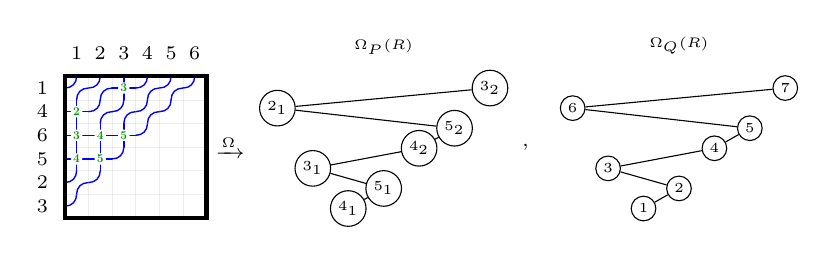
\begin{tikzpicture}[scale=0.3,
  tnode/.style={circle, draw=black, fill=white, inner sep=1.5pt, font=\tiny}]
  \draw[lightgray, very thin, opacity=0.3] (0,0) -- (6,0);
  \draw[lightgray, very thin, opacity=0.3] (0,0) -- (0,6);
  \draw[lightgray, very thin, opacity=0.3] (0,1) -- (6,1);
  \draw[lightgray, very thin, opacity=0.3] (1,0) -- (1,6);
  \draw[lightgray, very thin, opacity=0.3] (0,2) -- (6,2);
  \draw[lightgray, very thin, opacity=0.3] (2,0) -- (2,6);
  \draw[lightgray, very thin, opacity=0.3] (0,3) -- (6,3);
  \draw[lightgray, very thin, opacity=0.3] (3,0) -- (3,6);
  \draw[lightgray, very thin, opacity=0.3] (0,4) -- (6,4);
  \draw[lightgray, very thin, opacity=0.3] (4,0) -- (4,6);
  \draw[lightgray, very thin, opacity=0.3] (0,5) -- (6,5);
  \draw[lightgray, very thin, opacity=0.3] (5,0) -- (5,6);
  \draw[lightgray, very thin, opacity=0.3] (0,6) -- (6,6);
  \draw[lightgray, very thin, opacity=0.3] (6,0) -- (6,6);
  \draw[blue, line width=0.5pt] (0,5.5) .. controls (0.3,5.5) and (0.5,5.7) .. (0.5,6);
  \draw[blue, line width=0.5pt] (0.5,5) .. controls (0.5,5.3) and (0.7,5.5) .. (1,5.5);
  \draw[blue, line width=0.5pt] (1,5.5) .. controls (1.3,5.5) and (1.5,5.7) .. (1.5,6);
  \draw[blue, line width=0.5pt] (1.5,5) .. controls (1.5,5.3) and (1.7,5.5) .. (2,5.5);
  \draw[blue, line width=0.5pt, line cap=round] (2,5.5) -- (3,5.5);
  \draw[blue, line width=0.5pt, line cap=round] (2.5,5) -- (2.5,6);
  \draw[blue, line width=0.5pt] (3,5.5) .. controls (3.3,5.5) and (3.5,5.7) .. (3.5,6);
  \draw[blue, line width=0.5pt] (3.5,5) .. controls (3.5,5.3) and (3.7,5.5) .. (4,5.5);
  \draw[blue, line width=0.5pt] (4,5.5) .. controls (4.3,5.5) and (4.5,5.7) .. (4.5,6);
  \draw[blue, line width=0.5pt] (4.5,5) .. controls (4.5,5.3) and (4.7,5.5) .. (5,5.5);
  \draw[blue, line width=0.5pt] (5,5.5) .. controls (5.3,5.5) and (5.5,5.7) .. (5.5,6);
  \draw[blue, line width=0.5pt, line cap=round] (0,4.5) -- (1,4.5);
  \draw[blue, line width=0.5pt, line cap=round] (0.5,4) -- (0.5,5);
  \draw[blue, line width=0.5pt] (1,4.5) .. controls (1.3,4.5) and (1.5,4.7) .. (1.5,5);
  \draw[blue, line width=0.5pt] (1.5,4) .. controls (1.5,4.3) and (1.7,4.5) .. (2,4.5);
  \draw[blue, line width=0.5pt] (2,4.5) .. controls (2.3,4.5) and (2.5,4.7) .. (2.5,5);
  \draw[blue, line width=0.5pt] (2.5,4) .. controls (2.5,4.3) and (2.7,4.5) .. (3,4.5);
  \draw[blue, line width=0.5pt] (3,4.5) .. controls (3.3,4.5) and (3.5,4.7) .. (3.5,5);
  \draw[blue, line width=0.5pt] (3.5,4) .. controls (3.5,4.3) and (3.7,4.5) .. (4,4.5);
  \draw[blue, line width=0.5pt] (4,4.5) .. controls (4.3,4.5) and (4.5,4.7) .. (4.5,5);
  \draw[blue, line width=0.5pt, line cap=round] (0,3.5) -- (1,3.5);
  \draw[blue, line width=0.5pt, line cap=round] (0.5,3) -- (0.5,4);
  \draw[blue, line width=0.5pt, line cap=round] (1,3.5) -- (2,3.5);
  \draw[blue, line width=0.5pt, line cap=round] (1.5,3) -- (1.5,4);
  \draw[blue, line width=0.5pt, line cap=round] (2,3.5) -- (3,3.5);
  \draw[blue, line width=0.5pt, line cap=round] (2.5,3) -- (2.5,4);
  \draw[blue, line width=0.5pt] (3,3.5) .. controls (3.3,3.5) and (3.5,3.7) .. (3.5,4);
  \draw[blue, line width=0.5pt, line cap=round] (0,2.5) -- (1,2.5);
  \draw[blue, line width=0.5pt, line cap=round] (0.5,2) -- (0.5,3);
  \draw[blue, line width=0.5pt, line cap=round] (1,2.5) -- (2,2.5);
  \draw[blue, line width=0.5pt, line cap=round] (1.5,2) -- (1.5,3);
  \draw[blue, line width=0.5pt] (2,2.5) .. controls (2.3,2.5) and (2.5,2.7) .. (2.5,3);
  \draw[blue, line width=0.5pt] (0,1.5) .. controls (0.3,1.5) and (0.5,1.7) .. (0.5,2);
  \draw[blue, line width=0.5pt] (0.5,1) .. controls (0.5,1.3) and (0.7,1.5) .. (1,1.5);
  \draw[blue, line width=0.5pt] (1,1.5) .. controls (1.3,1.5) and (1.5,1.7) .. (1.5,2);
  \draw[blue, line width=0.5pt] (0,0.5) .. controls (0.3,0.5) and (0.5,0.7) .. (0.5,1);
  \node[font=\scriptsize, text=black, anchor=east] at (-0.3,5.5) {1};
  \node[font=\scriptsize, text=black, anchor=east] at (-0.3,4.5) {4};
  \node[font=\scriptsize, text=black, anchor=east] at (-0.3,3.5) {6};
  \node[font=\scriptsize, text=black, anchor=east] at (-0.3,2.5) {5};
  \node[font=\scriptsize, text=black, anchor=east] at (-0.3,1.5) {2};
  \node[font=\scriptsize, text=black, anchor=east] at (-0.3,0.5) {3};
  \node[font=\scriptsize, text=black, anchor=south] at (0.5,6.3) {1};
  \node[font=\scriptsize, text=black, anchor=south] at (1.5,6.3) {2};
  \node[font=\scriptsize, text=black, anchor=south] at (2.5,6.3) {3};
  \node[font=\scriptsize, text=black, anchor=south] at (3.5,6.3) {4};
  \node[font=\scriptsize, text=black, anchor=south] at (4.5,6.3) {5};
  \node[font=\scriptsize, text=black, anchor=south] at (5.5,6.3) {6};
  \node[font=\Large\bfseries, text=green!60!black, fill=white, inner sep=0.5pt, circle, transform shape] at (2.5,5.5) {3};
  \node[font=\Large\bfseries, text=green!60!black, fill=white, inner sep=0.5pt, circle, transform shape] at (0.5,4.5) {2};
  \node[font=\Large\bfseries, text=green!60!black, fill=white, inner sep=0.5pt, circle, transform shape] at (2.5,3.5) {5};
  \node[font=\Large\bfseries, text=green!60!black, fill=white, inner sep=0.5pt, circle, transform shape] at (1.5,3.5) {4};
  \node[font=\Large\bfseries, text=green!60!black, fill=white, inner sep=0.5pt, circle, transform shape] at (0.5,3.5) {3};
  \node[font=\Large\bfseries, text=green!60!black, fill=white, inner sep=0.5pt, circle, transform shape] at (1.5,2.5) {5};
  \node[font=\Large\bfseries, text=green!60!black, fill=white, inner sep=0.5pt, circle, transform shape] at (0.5,2.5) {4};
  \draw[black, line width=1.5pt] (0,0) rectangle (6,6);
  % Arrow between pipe dream and trees
  \node[font=\scriptsize] at (7, 3) {$\xrightarrow{\Omega}$};
  % LBS tree (inorder x-positions * 1.5 + 8.5, depth-based y)
  % inorder: N2=1, N3=2, N4=3, N5=4, N6=5, N7=6, N8=7
  % depth:   N8=0, N2=1, N7=2, N6=3, N3=4, N5=5, N4=6
  \node[font=\tiny\itshape, anchor=south] at (13.5,6.5) {$\Omega_P(R)$};
  \node[tnode] (lbs8) at (18.0, 5.5)  {$3_2$};
  \node[tnode] (lbs2) at (9.0,  4.65) {$2_1$};
  \node[tnode] (lbs7) at (16.5, 3.8)  {$5_2$};
  \node[tnode] (lbs6) at (15.0, 2.95) {$4_2$};
  \node[tnode] (lbs3) at (10.5, 2.1)  {$3_1$};
  \node[tnode] (lbs5) at (13.5, 1.25) {$5_1$};
  \node[tnode] (lbs4) at (12.0, 0.4)  {$4_1$};
  \draw (lbs8) -- (lbs2);
  \draw (lbs2) -- (lbs7);
  \draw (lbs7) -- (lbs6);
  \draw (lbs6) -- (lbs3);
  \draw (lbs3) -- (lbs5);
  \draw (lbs5) -- (lbs4);
  % Separator
  \node[font=\scriptsize] at (19.5, 3) {,};
  % Dec tree (offset 12 more in x: 8.5+12=20.5)
  \node[font=\tiny\itshape, anchor=south] at (26.0,6.5) {$\Omega_Q(R)$};
  \node[tnode] (dec8) at (30.5, 5.5)  {$7$};
  \node[tnode] (dec2) at (21.5, 4.65) {$6$};
  \node[tnode] (dec7) at (29.0, 3.8)  {$5$};
  \node[tnode] (dec6) at (27.5, 2.95) {$4$};
  \node[tnode] (dec3) at (23.0, 2.1)  {$3$};
  \node[tnode] (dec5) at (26.0, 1.25) {$2$};
  \node[tnode] (dec4) at (24.5, 0.4)  {$1$};
  \draw (dec8) -- (dec2);
  \draw (dec2) -- (dec7);
  \draw (dec7) -- (dec6);
  \draw (dec6) -- (dec3);
  \draw (dec3) -- (dec5);
  \draw (dec5) -- (dec4);
\end{tikzpicture}
\end{center}

\end{frame}

\begin{frame}{Algebra of forest pipe dreams}
    \begin{theorem}[S, 2026+]
    $\Omega\RC$ inherits the product $\star$ from $\RC$ via the function $R\mapsto [R]$ from the subalgebra of $\RC$ generated by the pipe dreams satisfying $\code(\Omega(R))=\code(\mathrm{perm}(R))$, which is a surjective homomorphism of rings onto $\Omega\RC$. The function
    $$\pi_{\Forest{}}:\Omega\RC\to\dcoma$$
    such that
    $$[R]\mapsto \Forest{\mathrm{code}(\Omega(R))}^*$$
    is a surjective homomorphism of rings onto $\dcoma$.
    \end{theorem}
\end{frame}

\begin{frame}{Dual forest LR rule/branching formula}
  \begin{theorem}[S, 2026+]
    Suppose
    
    $$\Forest{F}^*\Forest{G}^* = \sum_H f_{F,G}^H \Forest{H}^*$$
    where $f_{F,G}^H$ are the structure constants for the product in $\dcoma$. Then $f_{F,G}^H$ counts the sum of the coefficients of all $[R_H]$ such that $\code(\Omega(R_H))=H$ in a product $[R_F]\star [R_G]\in\Omega\RC$ with $\code(\Omega(R_F)) = F$ and $\code(\Omega(R_G)) = G$, and in particular is nonnegative.
  \end{theorem}
  
\end{frame}

\begin{frame}{Dual forest polynomial coproduct?}
  It is known (combinatorially, but not with a formula) that forest polynomials have nonnegative structure constants, so that dual forest polynomials $\Forest{F}^*$ have nonnegative structure constants for the coproduct in $\dcoma$. 
  
  For example,
  \begin{align*}
    \Delta\!\left(\Forest{1,2}^*\right) =\;
      &\Forest{0,0}^*\!\otimes\!\Forest{1,2}^*
      + \Forest{0,1}^*\!\otimes\!\Forest{0,2}^*
      + \Forest{0,1}^*\!\otimes\!\Forest{1,1}^*
      + \Forest{0,2}^*\!\otimes\!\Forest{0,1}^* \\
      +\;&\Forest{0,2}^*\!\otimes\!\Forest{1,0}^*
      + \Forest{1,0}^*\!\otimes\!\Forest{0,2}^*
      + \Forest{1,1}^*\!\otimes\!\Forest{0,1}^*
      + \Forest{1,2}^*\!\otimes\!\Forest{0,0}^*
  \end{align*}
  \begin{itemize}
  \item It is distinctly possible that a positive coproduct formula for $\Forest{F}^*$ in $\dcoma$ can be obtained by analyzing the $\star$ product of pipe dreams with $F(R) = F$.
  \end{itemize}
\end{frame}

\begin{frame}{Summary}
  \begin{itemize}
    \item The pipe dream ring $\RC$ with product $\star$ lifts the algebra $\dcoma$ and gives positive LR rules for dual Schubert, key, and forest polynomials by taking appropriate quotients of subalgebras.
    \item The forest coproduct story (branching formula) is an active direction.
  \end{itemize}
  \vspace{0.5em}
  \centering Thank you!
\end{frame}

\begin{frame}[allowframebreaks]{References}
  \bibliographystyle{plain}
  \bibliography{molev-sagan-paper}
\end{frame}

\end{document}
